\documentclass[a4paper,10pt]{book}

\usepackage[usenames]{color}
\usepackage{bm}
\usepackage{amsmath}
\usepackage{xspace}
\usepackage{a4wide}
\usepackage{wrapfig}
\usepackage[numbers,comma,sort&compress]{natbib}
\usepackage{graphicx}
\usepackage{xstring}
\usepackage{listings,courier}
%\usepackage{draftcopy}
\usepackage{longtable}
\usepackage{paralist}
%\usepackage{fancyvrb}
\usepackage{listings}
\usepackage{array}
\usepackage[table]{xcolor}
\usepackage{units}
\usepackage[toc,page]{appendix}

\definecolor{webgreen}{rgb}{0,.5,0}
\definecolor{webbrown}{rgb}{.6,0,0}
\definecolor{invisiblegray}{rgb}{.97,0.97,0.97}

\usepackage
[dvips, %dvipdf, %or dvips or pdftex 
pagebackref, %or backref
colorlinks=true,
linkcolor=webgreen, %defined below
filecolor=webbrown, %defined below
citecolor=webgreen, %defined below
pdftitle={VOTCA-CT manual},
pdfauthor={},
pdfsubject={VOTCA-CTP},
pdfkeywords={charge transport organic semiconductors},
bookmarksopen=false,
pdfpagemode=UseNone]{hyperref}

%\pdfcompresslevel=9

\usepackage[T1]{fontenc}
%\usepackage{times}
\usepackage{type1cm}

\def\bibsection{%
    \chapter*{Bibliography}%
    \addcontentsline{toc}{chapter}{Bibliography}
}

\begin{document}


\lstset{
  language=XML,
  frame=lines,
  backgroundcolor=\color{invisiblegray},
  basicstyle=\ttfamily\footnotesize,
  identifierstyle=\color{red},
  keywordstyle=\color{blue},
  commentstyle=\color{gray}\rmfamily\itshape,
  mathescape=true,
  morekeywords={estatic_params,estatic_method,epsilon_dielectric,s_eps}
}

\input{hgid}

\newcommand{\equ}[1]{eq.~\eqref{equ:#1}}
\newcommand{\Equ}[1]{Eq.~\eqref{equ:#1}}
\newcommand{\fig}[1]{figure~\ref{fig:#1}}
\newcommand{\Fig}[1]{Figure~\ref{fig:#1}}
\newcommand{\sect}[1]{section~\ref{sec:#1}}

\newcommand{\slink}[2]{\hyperref[#1]{#2}}


\newcommand{\xml}{XML\xspace}
\newcommand{\gromacs}{GROMACS\xspace}
\newcommand{\gaussian}{GAUSSIAN\xspace}
\newcommand{\turbomole}{TURBOMOLE\xspace}
\newcommand{\tinker}{TINKER\xspace}
\newcommand{\dipro}{DIPRO\xspace}

\newcommand{\Alq}{$\mathrm{Alq}_3$\xspace}
\newcommand{\dcvt}{DCV2T\xspace}

\newcommand{\xyz}{\texttt{geometry.xyz}\xspace}
\newcommand{\orb}{\texttt{zindo.orb}\xspace}
\newcommand{\votcactp}{{\MakeUppercase{votca-ctp}}\xspace}

\newcommand{\calculator}{\hyperref[sec:calculators]{calculator}\xspace}

\newcommand{\xmloptions}{\texttt{options.xml}\xspace}
\newcommand{\xmlcsg}{\hyperref[sec:xmlmap]{\texttt{map.xml}}\xspace}
\newcommand{\xmlsegments}{\hyperref[sec:xmlsegments]{\texttt{segments.xml}}\xspace}
\newcommand{\sqlstate}{\hyperref[sec:statefile]{\texttt{state.db}}\xspace}
\newcommand{\topology}{\texttt{topol.tpr}\xspace}
\newcommand{\trajectory}{\texttt{traj.xtc}\xspace}

\newcommand{\opt}{\texttt{{ -}o}\xspace}
\newcommand{\seg}{\texttt{{ -}s}\xspace}
\newcommand{\sql}{\texttt{{ -}f}\xspace}
\newcommand{\exe}{\texttt{{ -}e}\xspace}
\newcommand{\tpl}{\texttt{{ -}t}\xspace}
\newcommand{\csg}{\texttt{{ -}m}\xspace}
\newcommand{\trj}{\texttt{{ -}c}\xspace}


\newcommand{\refcalc}{\hyperref[ref:calculators]{calculators}\xspace}

\newcommand{\overlap}{\hyperref[prog:moo_overlap]{\texttt{moo\_overlap}}\xspace}
\newcommand{\ctprun}{\hyperref[prog:ctp_run]{\texttt{ctp\_run}}\xspace}
\newcommand{\ctpmap}{\hyperref[prog:ctp_map]{\texttt{ctp\_map}}\xspace}
\newcommand{\ctpdipro}{\hyperref[prog:ctp_dipro]{\texttt{ctp\_dipro}}\xspace}

\newcommand{\sqlite}{\texttt{sqlite3}\xspace}
\newcommand{\sqlconjsegproperties}{\texttt{conjseg\_properties}\xspace}
\newcommand{\sqlconjsegs}{\texttt{conjsegs}\xspace}
\newcommand{\sqlmolecules}{\texttt{molecules}\xspace}
\newcommand{\sqlpairintegrals}{\texttt{pairintegrals}\xspace}
\newcommand{\sqlpairproperties}{\texttt{pairproperties}\xspace}
\newcommand{\sqlpairs}{\texttt{pairs}\xspace}
\newcommand{\sqlrigidfragproperties}{\texttt{rigidfrag\_properties}\xspace}
\newcommand{\sqlrigidfrags}{\texttt{rigidfrags}\xspace}
\newcommand{\sqlframes}{\texttt{frames}\xspace}


\newcommand{\suggestion}[1]{{\color{red}SUGGESTION: #1}}

\newcommand{\segmentref}[1]{segments.#1}
\newcommand{\segmentopt}[1]{\hyperlink{\segmentref{#1}}{\StrSubstitute{#1}{_}{\_}}\xspace}
\newcommand{\calcref}[1]{#1}
\newcommand{\calcopt}[1]{\hyperlink{\calcref{#1}}{\StrSubstitute{#1}{_}{\_}}\xspace}

\newcommand{\calc}[1]{\hyperref[calc:#1]{\texttt{#1}}\xspace}

\def\bibsection{%
    \chapter*{Bibliography}%
    \addcontentsline{toc}{chapter}{Bibliography}
}

\renewcommand*{\showkeyslabelformat}[1]{{\normalfont\tiny\sffamily#1}}
\definecolor{refkey}{rgb}{1,0,0}
\definecolor{labelkey}{rgb}{1,0,0}


\frontmatter
\begin{titlepage}

\center{\fontsize{4cm}{5cm}\selectfont VOTCA}
\center{\fontsize{1.5cm}{3cm}\selectfont USER MANUAL}

\vspace*{3cm}
\center{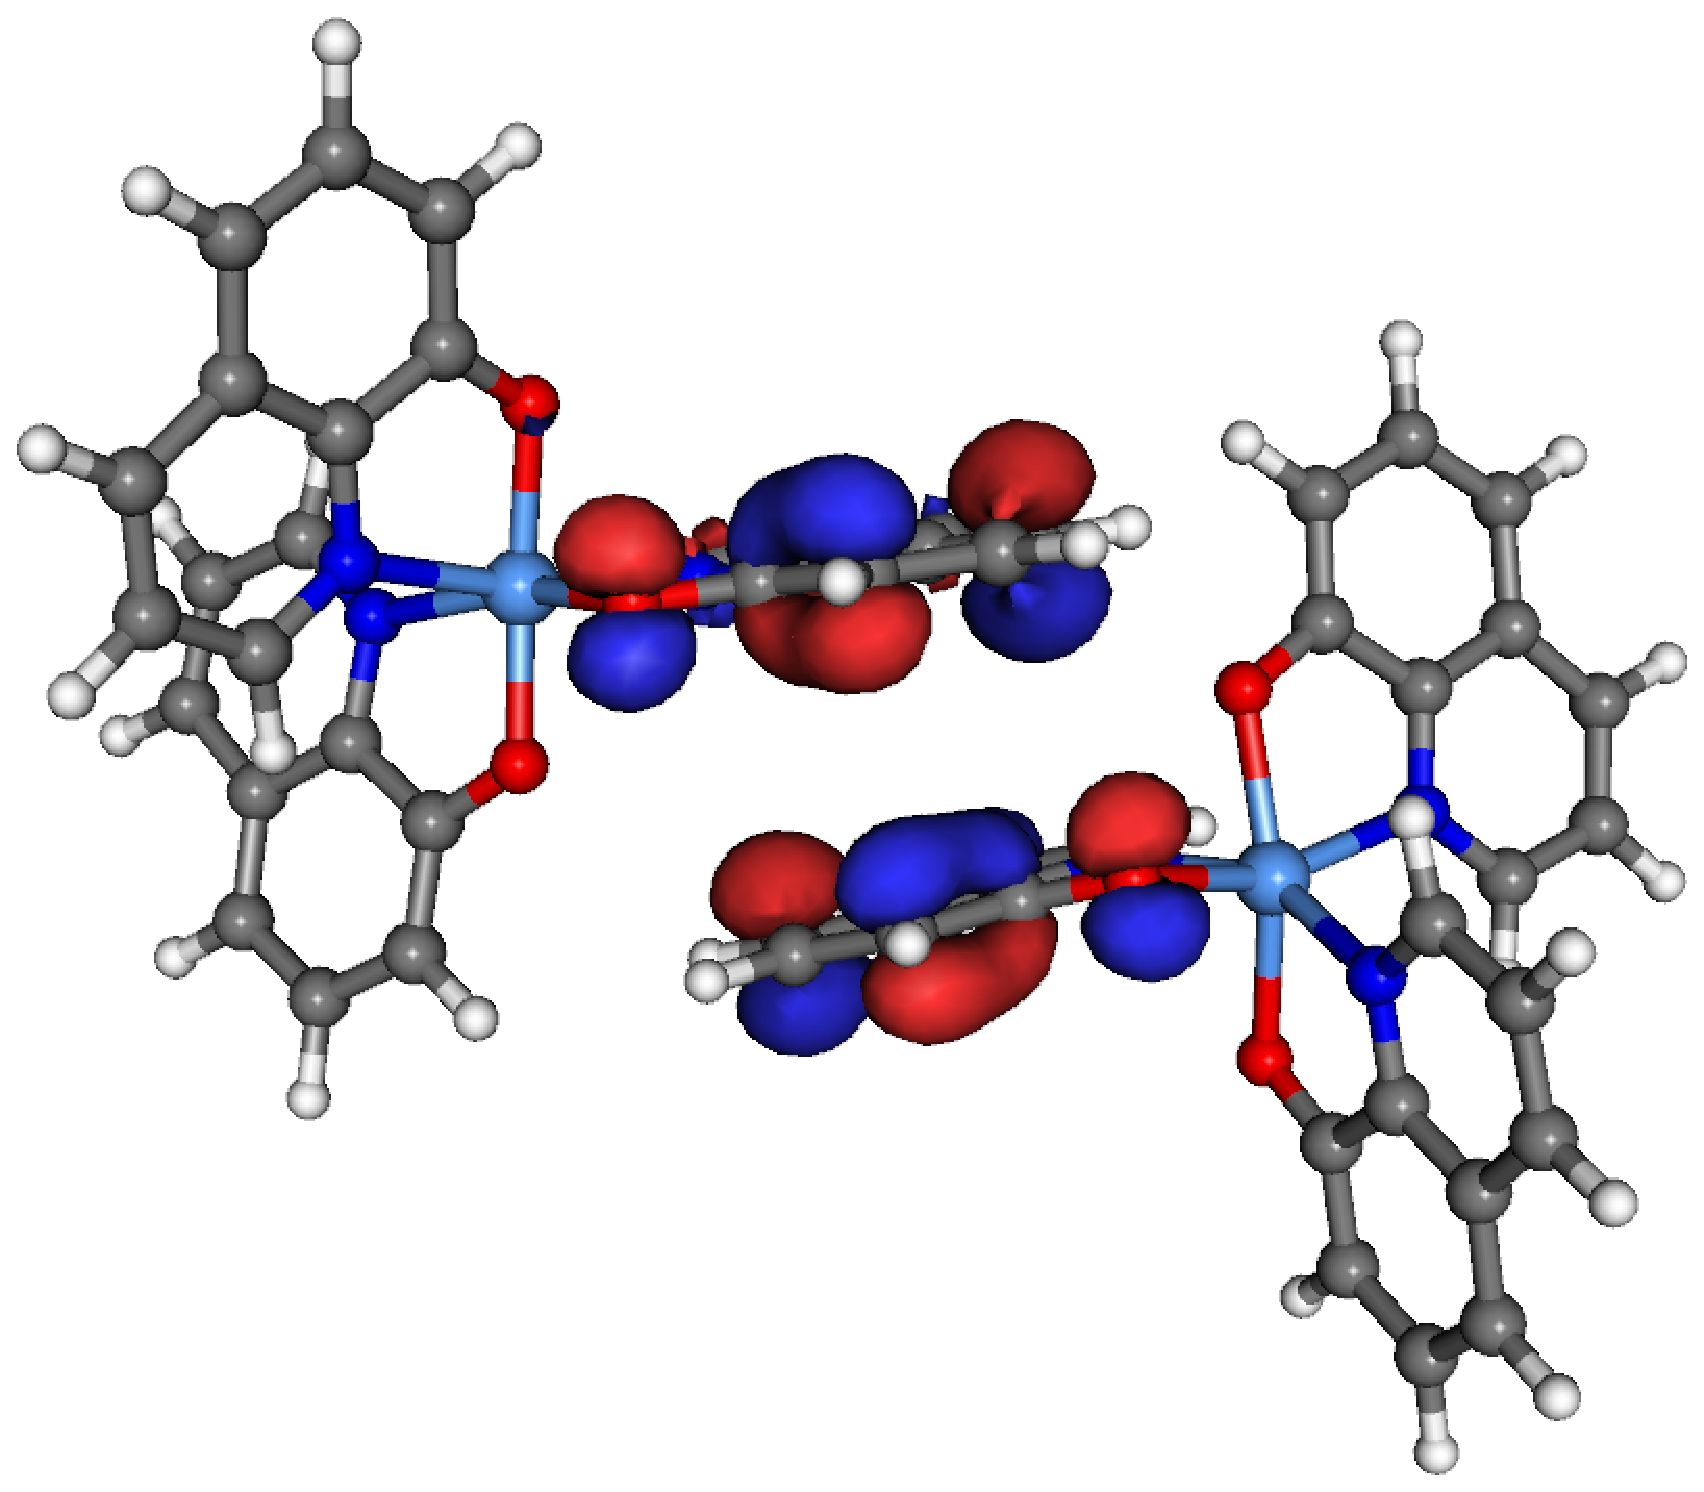
\includegraphics[width=\columnwidth]{fig/logo}}
\vspace*{1cm}
\vfill
\vspace*{1.4cm}
\center{\large{\today}}
\vspace*{-0.3cm}
\center{\footnotesize{Version: \gitid}}
\center{\footnotesize{Programs version: \csgid}}

\vspace*{1cm}
%\center{
\large{\copyright \hspace*{0.1cm} VOTCA development team}
%}
\vspace*{0.5cm}

\htmladdnormallink{\color{black}\large{www.votca.org}}{http://www.votca.org}
\end{titlepage}

\section*{Disclamer}
This manual is not complete. The best way to start using the software is to look at provided tutorials. The reference section is generated automatically from the source code, so please make sure that your software and manual versions match.  

\section*{Citations}
Development of this software depends on academic research grants. If you are using the package, please cite the  following papers \\

\vspace{0.1cm}
\noindent
\cite{mashayakrelative} Relative entropy and optimization-driven coarse-graining methods in VOTCA, \\
S.Y. Mashayak, Mara Jochum, Konstantin Koschke, N.R. Aluru, Victor R\"uhle, and Christoph Junghans,\\
\htmladdnormallink{  {\itshape Plos One} (2015)}
{http://dx.doi.org/10.1371/journal.pone.0131754}

\vspace{0.1cm}
\noindent
\cite{ruhle2011hybrid} Hybrid approaches to coarse-graining using the VOTCA package: liquid hexane, \\
Victor R\"uhle and Christoph Junghans, \\
\htmladdnormallink{  {\itshape Macromol. Theory Simul.} 20, 472 (2011)}
{http://dx.doi.org/10.1002/mats.201100011}

\vspace{0.1cm}
\noindent
\cite{Ruehle:2009.a} Versatile Object-oriented Toolkit for Coarse-graining Applications \\
Victor R\"uhle, Christoph Junghans, Alexander Lukyanov, Kurt Kremer, and Denis Andrienko \\
\htmladdnormallink{  {\itshape J. Chem. Theor. Comp.} 5, 3211, 2009}
{http://dx.doi.org/10.1021/ct900369w}

\section*{Development}
The core development is currently taking place at the Los Alamos National Laboratory and Max Planck Institute for Polymer Research, Mainz, Germany.

\section*{Copyright}
\votca is free software. The entire package is available under the Apache License. For details, check
the LICENSE file in the source code. The \votca source code is available on our homepage, \htmladdnormallink{\color{black}www.votca.org}{http://www.votca.org}.

\vfill

\thispagestyle{empty}
\cleardoublepage

\tableofcontents
%\cleardoublepage
\mainmatter
\chapter{Introduction}
\label{sec:introduction}

Charge carrier dynamics in an organic semiconductor can often be described in terms of charge hopping between localized states. The hopping rates depend on electronic coupling elements, reorganization energies, and driving forces, which vary as a function of position and orientation of the molecules.  The exact evaluation of these contributions in a molecular assembly is computationally prohibitive. Various, often semi-empirical, approximations are employed instead. The purpose of \votcactp is to simplify the workflow for charge transport simulations, provide a uniform error-control for the methods, flexible platform for their development, and eventually allow in silico pre-screening of organic semiconductors for specific applications. 

The toolkit is implemented using modular concepts introduced earlier in the Versatile Object-oriented Toolkit for Coarse-graining Applications (VOTCA)~\cite{ruehle_versatile_2009}. The VOTCA structures are adapted to reading atomistic trajectories, mapping them onto conjugated segments and rigid fragments, and substituting (if needed) rigid fragments with the optimized copies. 

The \hyperref[sec:moo]{molecular orbital overlap} module calculates electronic coupling elements between  conjugated segments from the corresponding molecular orbitals. It relies on the semi-empirical INDO Hamiltonian and molecular orbitals in the format provided by the \gaussian package. An alternative,  \hyperref[sec:dft]{density-functional based approach}, has interfaces to the \gaussian and \turbomole packages. An interface to the \tinker package is provided for calculations of electrostatic and polarization contributions to energetic disorder. 

The  \hyperref[sec:kmc]{kinetic Monte Carlo module} reads in the neighbor list, site coordinates, and hopping rates and performs charge dynamics simulations using either periodic boundary conditions or charge sources and sinks. 

The toolkit is written as a combination of modular C++ code and scripts. The data transfer between programs is implemented via a state file or database, which is also used to restart simulations. Analysis functions and most of the calculation routines are encapsulated by using the observer pattern~\cite{gamma_design_1995} which allows the implementation of new functions as individual modules.

\chapter{Theoretical background}
\label{sec:theory}
\section{Workflow}
\label{sec:wokflow}

A typical workflow of charge transport simulations is depicted in \fig{workflow}. The first step is the simulation of an \slink{morphology}{atomistic morphology}, which is then partitioned on \slink{segments}{hopping sites}. The coordinates of the hopping sites are used to construct a list of pairs of molecules, or \slink{neighborlist}{neighbor list}. 

\begin{figure}[h]
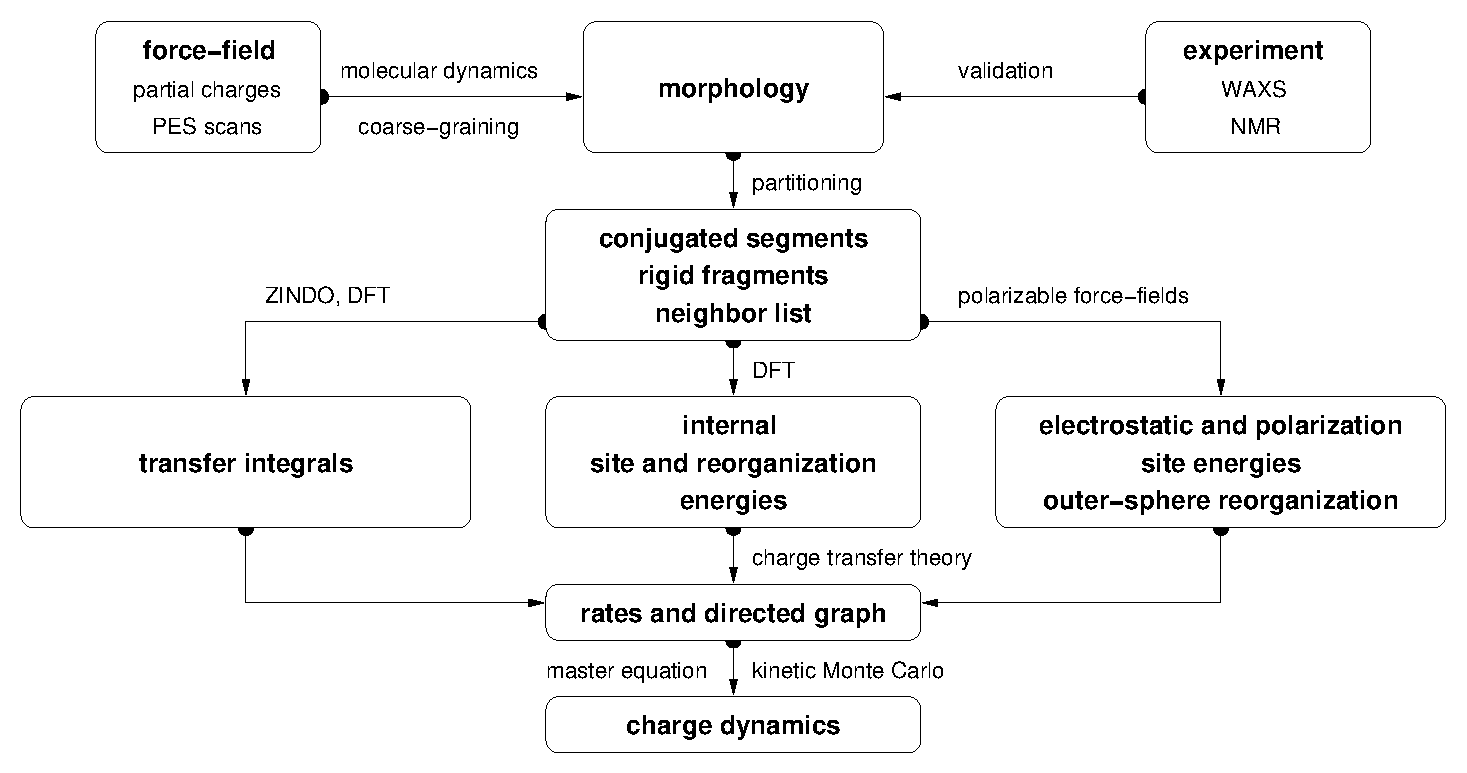
\includegraphics[width=\textwidth]{fig/workflow/workflow}
 \caption{%
   Workflow for microscopic simulations of charge transport.  %
   \label{fig:workflow}}
\end{figure}

For each pair an \slink{transfer_integrals}{electronic coupling element}, a \slink{reorganization}{reorganization energy}, a \slink{site_energies}{driving force}, and eventually the \slink{rates}{hopping rate} are evaluated. The neighbor list and hopping rates define a directed graph. The corresponding master equation is solved using the \slink{kmc}{kinetic Monte Carlo} method, which allows to explicitly monitor the charge dynamics in the system as well as to calculate time or ensemble averages of occupation probabilities, charge fluxes, correlation functions, and field-dependent mobilities.


\begin{figure}[p]
\includegraphics[width=\textwidth]{fig/workflow_practical/workflow_practical}
 \caption{%
   Workflow for microscopic simulations of charge transport including calls.  %
   \label{fig:workflow}}
\end{figure}


\tikzstyle{decision} = [diamond, draw, fill=blue!50]
\tikzstyle{line} = [draw, -stealth, thick]
\tikzstyle{elli}=[draw, ellipse, fill=red!50,minimum height=8mm, text width=5em ]
\tikzstyle{block} = [draw, rectangle, fill=blue!50, text width=\linewidth]
\tikzstyle{smallblock} = [draw, rectangle, fill=blue!50, text width=0.4\linewidth]
\begin{figure}
\centering
\newcommand{\vgap}{0.5cm}
\begin{footnotesize}
\noindent\begin{tikzpicture}
\node [block] (mapping) {{\bf Mapping}\\Converts and partitions atomistic \gromacs trajectory \vskip 0.1cm
{\noindent  \ctpmap \tpl \topology \trj \trajectory \seg \xmlcsg  \sql \sqlstate}
\vskip 0.1cm};

\node [block, below=\vgap of mapping] (nbl) {{\bf Neighbor list}\\Indentifies close molecular pairs between which charge transfer rates will be calculated \vskip 0.1cm
{\noindent  \ctprun \opt \xmloptions  \seg  \xmlsegments \sql  \sqlstate \exe  \calc{neighborlist}}
\vskip 0.1cm};


\node [block, below=\vgap of nbl] (site_energies) {{\bf Site energies}\\Calculates electrostatic and polarization contribution to site energies \vskip 0.1cm
{\noindent  \ctprun \opt \xmloptions  \sql  \sqlstate \exe  \calc{emultipole} } };

\node [block, below=\vgap of site_energies] (int_energies) {{\bf Internal site and reorganization energies}\\Imports internal site energy (IP, EA) and reorganization energies for charging and discharging to \sqlstate \vskip 0.1cm
{\noindent  \ctprun \opt \xmloptions  \sql  \sqlstate \exe  \calc{einternal} }
\vskip 0.1cm};


% above right=0.7cm and 4cm of A
\node[decision, below=\vgap of int_energies](decision1){Transfer integrals};

%\node (AuxNode01) [text width=6em, below of = decision1, node distance=7em ] {};

\node [smallblock, below left=\vgap of decision1] (DFT_TI) {{\bf Monomers with DFT}\\Calculate the relevant transport orbitals of monomers\\ prepare job file \vskip 0.1cm
{ \ctpparallel \opt \xmloptions \sql \sqlstate \exe \calc{edft} \job \wrt }
\vskip 0.1cm execute jobs \vskip 0.1cm
{ \ctpparallel \opt \xmloptions \sql \sqlstate \exe \calc{edft} \job \run }
};

\node [smallblock, below=\vgap of DFT_TI] (DFT_TI2) {{\bf Electronic coupling with DFT}\\Calculate electronic coupling elements for all pairs in the neighbor list \vskip 0.1cm
{ \ctpparallel \opt \xmloptions \sql \sqlstate \exe \calc{idft} \job `` \wrt \run \rd\'' }
\vskip 0.1cm};

\node [smallblock, below right=\vgap of decision1] (DFT_ZINDO) {{\bf Electronic coupling with ZINDO}\\Imports internal site energy (IP, EA) and reorganization energies for charging and discharging to \sqlstate \vskip 0.1cm
{\noindent  \ctprun \opt \xmloptions  \sql  \sqlstate \exe  \calc{einternal} }
\vskip 0.1cm};

\node (AuxNode01) [below=\vgap of DFT_TI2, xshift=0.25\linewidth] {};


\node [block, below=\vgap of DFT_TI2, xshift=0.275\linewidth] (outer_reorg) {{\bf Outersphere reorganization energies}\\Imports internal site energy (IP, EA) and reorganization energies for charging and discharging to \sqlstate \vskip 0.1cm
{\noindent  \ctprun \opt \xmloptions  \sql  \sqlstate \exe  \calc{outersphere} }
\vskip 0.1cm};

\node [block, below=\vgap of outer_reorg] (rates) {{\bf Charge transfer rates}\\Calculates rates for charge transfer among all pairs in the neighborlist \vskip 0.1cm
{\noindent \small \ctprun \opt \xmloptions \sql  \sqlstate \exe  \calc{rates} }
};

\node [block, below=\vgap of rates] (kmc) {{\bf Charge dynamics via kMC}\\Hopping of charge carriers simulated via kinetic Monte Carlo \vskip 0.1cm
{\noindent  \kmcrun \opt \xmloptions  \sql  \sqlstate \exe  \calc{kmcmultiple} }
};
%%
%(ClOp.west) -- ++(-0.2,0) -- ([yshift=0.5cm, xshift=-0.2cm] Pressure.north west) -|
%     ([xshift=-1cm]Sensor.south);
%    \draw[myarrow] (Ammeter.east) -- ++(0.2,0) -- ([yshift=0.5cm, xshift=0.2cm] Temperature.north east) -|
%     ([xshift=1cm]Sensor.south);

%\node [block, left of=mapping, xshift=-5em] (nbl) {Process 1};
%\node [elli, above of=mapping, yshift=5em] (user) {user};
%\node [block, right of=mapping, xshift=5em] (process2) {Process 2};
%\node[decision, below of=mapping, yshift=-5em](decision1){Process 1?};
%arrows
%\path [line] (user) -- (mapping);
\path [line] (mapping) -- (nbl);
\path [line] (nbl) -- (site_energies);
\path [line] (site_energies) -- (int_energies);
\path [line] (int_energies) -- (decision1);
\path [line] (DFT_TI) -- (DFT_TI2);
\path [line] (decision1) -| node[yshift=0.5em, xshift=1em] {DFT} (DFT_TI);
\path [line] (decision1) -| node[yshift=0.5em, xshift=-1em] {ZINDO} (DFT_ZINDO);
\path [line] (DFT_TI2) -- (outer_reorg);
\path [line] (DFT_ZINDO) -- (outer_reorg);
\path [line] (outer_reorg) -- (rates);
\path [line] (rates) -- (kmc);
\end{tikzpicture}


\end{footnotesize}
\caption{LALA}
\end{figure}


\chapter{System morphology}
\label{sec:morphology}

In this section we describe how to specify the morphology of the system. We will use DCV2T as an example.

\section{Single molecule}

\begin{wrapfigure}{ht}{0.5\linewidth}
\centering
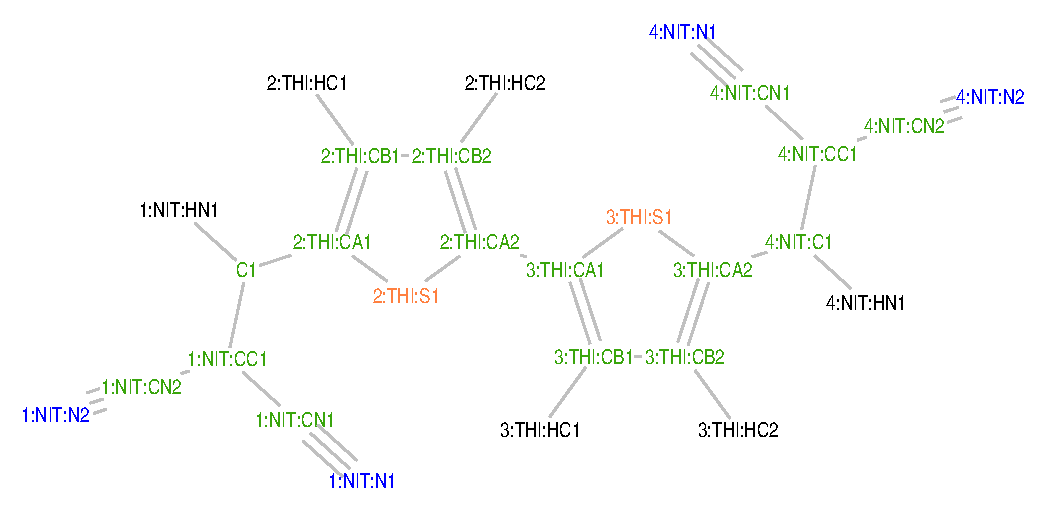
\includegraphics[width=0.9\linewidth]{./fig/chemical_structure/dcv2t_atom_types}
\caption{\small Atom types of DCV2T. The molecule consists of two building blocks (residues): thiophene (THI) and dicyanovinyl (NIT). }
\label{fig:dcv2t_at}
\end{wrapfigure}

%\clearpage
The structure of DCV2T, together with atom type definitions, is shown in fig.~\ref{fig:dcv2t_at}. DCV2T is a typical donor-acceptor-type molecule, with two electron-donating thiophene and two electron-withdrawing dicyanovinyl groups. The pdb file which contains residue types, residue numbering, atom names, atom types, and atom coordinates is shown below. In its ground state the molecule is practically planar. 

\section{Simulation box}
An amorphous morphology was obtained by quenching the 512 DCV2T molecules after equilibrating the system above the glass transition temperature. What we will need is a snapshot out of the trajectory and the topology file describing the system (all in GROMACS format).

\clearpage
\lstinputlisting[
  basicstyle=\ttfamily\footnotesize,
  frame=lines,
  identifierstyle=\color{red},
  keywordstyle=\color{blue},
  showstringspaces=false,
 label=list:pdb, 
 morekeywords={HETATM,THI,NIT},
 caption={pdb file of DCV2T}]%
{./fig/chemical_structure/dcv2t.pdb}

%\VerbatimInput[%
%frame=lines,
%framesep=4mm,
%label=\fbox{pdb file of DCV2T}, 
%framerule=0.5mm,
%rulecolor=\color{red},
%baselinestretch=1,
%fontsize=\footnotesize%,
%numbers=left
%]%
%{./fig/chemical_structure/dcv2t.pdb}

\section{Conjugated segments and rigid fragments}
\label{sec:segments}

\begin{figure}
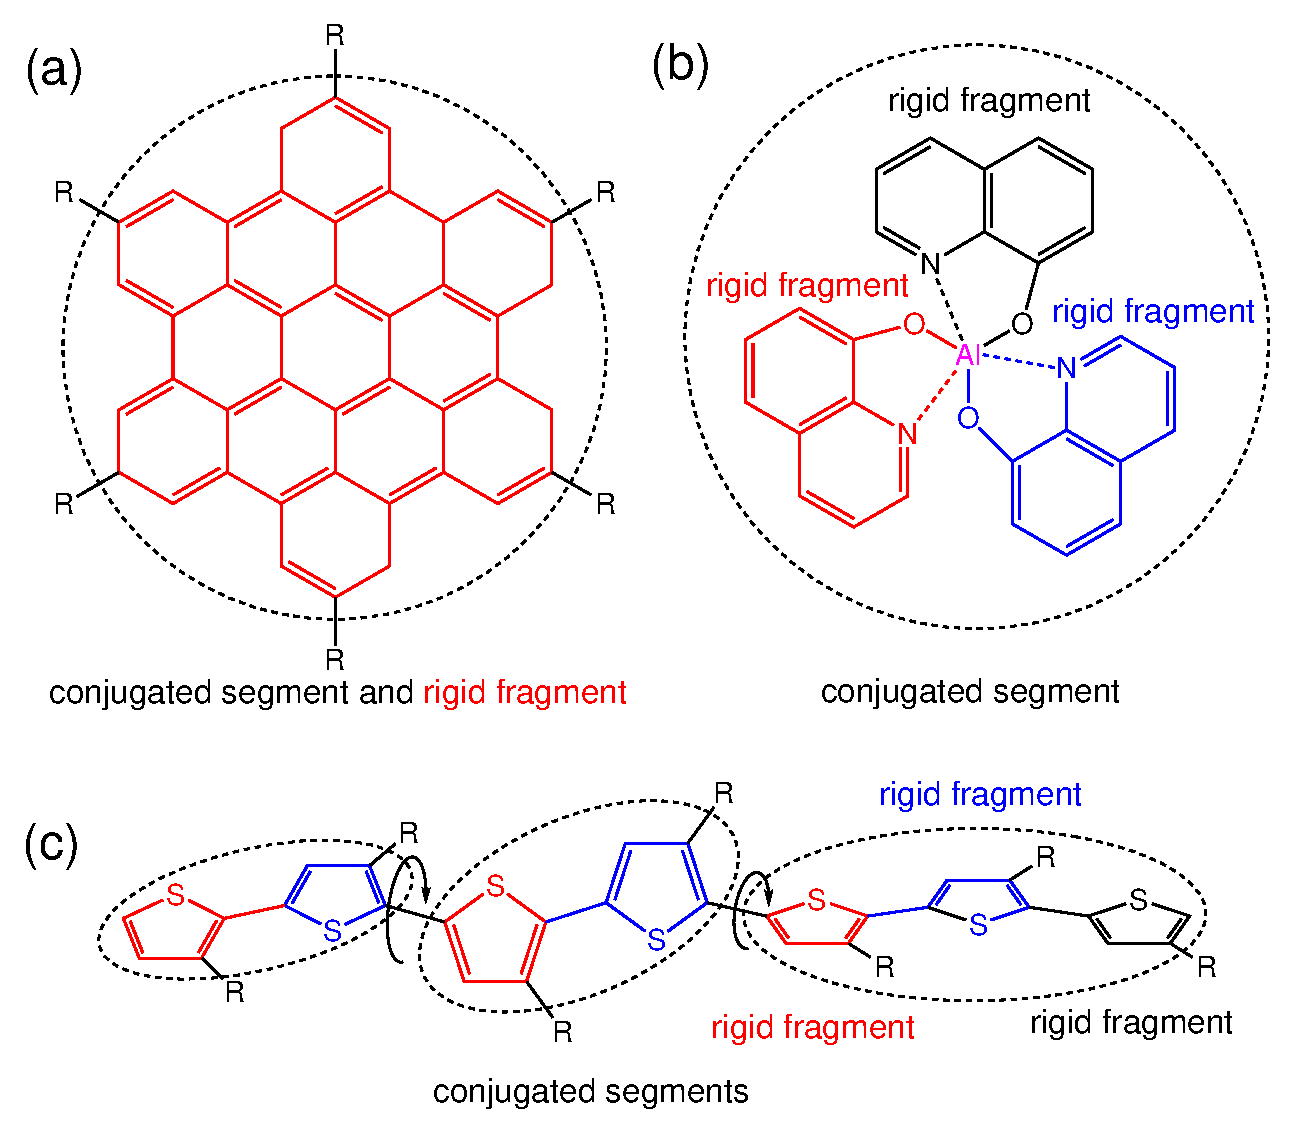
\includegraphics[width=\linewidth]{fig/conjugated_segment/fragment_segment}
\caption{The concept of conjugated segments and rigid fragments. Dashed lines indicate conjugated segments while colors denote rigid fragments. (a) Hexabenzocoronene: the $\pi$-conjugated system is both a rigid fragment and a conjugated segment. (b) \Alq: the Al atom and each ligand are rigid fragments while the whole molecule is a conjugated segment. (c) Polythiophene: each repeat unit is a rigid fragment. A conjugated segment consists of one or more rigid fragments. One molecule can have several conjugated segments.}
\label{fig:segment}
\end{figure}

With the morphology at hand, the next step is partitioning the system on hopping sites\index{hopping site}, or conjugated segments\index{conjugated segment}, and calculating charge transfer rates between them. Physically intuitive arguments can be used for the partitioning,  which reflects the localization of the wave function of a charge. For most organic semiconductors, the molecular architecture includes relatively rigid, planar $\pi$-conjugated systems, which we will refer to as rigid fragments. A conjugated segment can contain one or more of such rigid fragments, which are linked by bonded degrees of freedom. The dynamics of these degrees of freedom evolves on timescales much slower than the frequency of the internal promoting mode. In some cases, e.g. glasses, it can be `frozen' due to non-bonded interactions with the surrounding molecules.

To illustrate the concept of conjugated segments and rigid fragments, three representative molecular architectures are shown in \fig{segment}. The first one is a typical discotic liquid crystal, hexabenzocoronene. It consists of a conjugated core to which side chains are attached to aid self-assembly and solution processing. In this case the orbitals localized on side chains do not participate in charge transport and the conjugated $\pi$-system is both, a rigid fragment and a conjugated segment. 
%
In \Alq, a metal-coordinated compound, a charge carrier is delocalized over all three ligands. Hence, the whole molecule is one conjugated segment. Individual ligands are relatively rigid, while energies of the order of $k_\text{B}T$ are sufficient to reorient them with respect to each other. Thus the Al atom and the three ligands are rigid fragments.
%
In the case of a conjugated polymer, one molecule can consist of several conjugated segments, while each backbone repeat unit is a rigid fragment. Since the conjugation along the backbone can be broken due to large out-of-plane twists between two repeat units, an empirical criterion, based on the dihedral angle, can be used to partition the backbone on conjugated segments~\cite{ruhle_multiscale_2010}. However, such intuitive partitioning is, to some extent, arbitrary and shall be validated by other methods~\cite{vukmirovic_charge_2008,vukmirovic_charge_2009,mcmahon_ad_2009}. 

After partitioning, an additional step is often required to remove bond length fluctuations introduced by molecular dynamics simulations, since they are already integrated out in the derivation of the rate expression. This is achieved by substituting respective molecular fragments with  rigid, planar $\pi$-systems\index{rigid fragment} optimized using first-principles methods. Centers of mass and gyration tensors are used to align rigid fragments, though a custom definition of local axes is also possible. Such a procedure also minimizes discrepancies between the force-field and first-principles-based ground state geometries of conjugated segments, which might be important for calculations of electronic couplings, reorganization energies, and intramolecular driving forces. 

To partition the system on hopping sites and substitute rigid fragments with the corresponding ground-state geometries \ctpmap program is used:
\votcacommand{Mapping the \gromacs trajectory}{\cmdmap}
It reads in the \gromacs topology (\topology) and trajectory (\trajectory) files, definitions of conjugated segments and rigid fragments (\xmlcsg) and outputs coordinates of conjugated segments (hopping sites) and rigid fragments (as provided in the MD trajectory and after rigidification) to the  state file (\sqlstate). In order to do this, a mapping file \xmlcsg has to be provided, which specifies the corresponding atoms in the different representations. After this step, all information (frame number, dimensions of the simulation box, etc) are stored in the \slink{statefile}{state file} and only this file is used for further calculations.  

In order to visually check the mapping one can use either the \calc{tdump} \calculator or the programm \ctpdump with the calculator \calc{trajectory2pdb}.

\label{sec:ctp_dump}
\votcacommand{Writing a mapped trajectroy with \ctpdump}{\small \ctpdump \sql \sqlstate \exe \calc{trajectory2pdb} }

It reads in the state file created by \ctpmap and outputs two trajectory files corresponding to the original and rigidified atom coordinates. To check the mapping, it is useful to superimpose the three outputs (original atomistic, atomistic stored in the state file, and rigidified according to ground state geometries), e.g., with {\tt VMD}.

\label{sec:tdump}
\votcacommand{Writing a mapped trajectroy with \calc{tdump} }{\small \ctprun \sql \sqlstate \opt \xmloptions \exe \calc{tdump} }

It also reads in the state file but appends the coordinates to a pdb. file. So make sure to delete old QM.pdb and MD.pdb if you want to create a new imagef



\section{Neighbor list}
\label{sec:neighborlist}

A list of neigboring conjugated segments, or neighbor list\index{neighbor list}, contains all pairs of conjugated segments for which \slink{sec:transfer_integrals}{coupling elements}, \slink{sec:reorganization}{reorganization energies}, \slink{sec:site_energies}{site energy differences}, and \slink{sec:rates}{rates} are evaluated.

Two segments are added to this list if the distance between centers of mass of any of their rigid fragments is below a certain cutoff. This allows neighbors to be selected on a criterion of minimum distance of approach rather than center of mass distance, which is useful for molecules with anisotropic shapes.

The neighbor list can be generated from the atomistic trajectory by using the \calc{neighborlist} \calculator. This calculator requires a cutoff, which can be specified in the \xmloptions file. The list is saved to the \sqlstate file:
\votcacommand{Generating a neighbor list}{\cmdnbl}

\section{Reorganization energy}
\label{sec:reorganization}

The reorganization energy $\lambda_{ij}$ takes into account the change in  nuclear (and dielectric) degrees of freedom as the charge moves from donor $i$ to acceptor $j$. It has two contributions: intramolecular, $\lambda^\text{int}_{ij}$, which is due to reorganization of nuclear coordinates of the two molecules forming the charge transfer complex, and intermolecular (outer-sphere), $\lambda^\text{out}_{ij}$, which is due to the relaxation of the environment. In what follows we discuss how these contributions can be calculated.

\subsection{Intramolecular reorganization energy}
\label{sec:inner_reorganization}
If intramolecular vibrational modes of the two molecules are treated classically, the rearrangement of their nuclear coordinates after charge transfer results in the dissipation of the internal reorganization energy, $\lambda_{ij}^\text{int}$. It can be computed from four points on the potential energy surfaces (PES) of both molecules in neutral and charged states, as indicated in \fig{parabolas}. Adding the contributions due to discharging of molecule $i$ and charging of molecule $j$ yields~\cite{bredas_charge-transfer_2004}
\begin{equation}
\lambda_{ij}^\text{int} =\lambda_{i}^{cn}+\lambda_{j}^{nc}=U_{i}^{nC}-U_{i}^{nN}+U_{j}^{cN}-U_{j}^{cC}\,.
\label{equ:lambdas}
\end{equation}
Here $U_{i}^{nC}$ is the internal energy of the neutral molecule $i$ in the geometry of its charged state (small $n$ denotes the state and capital $C$ the geometry). Similarly, $U_{j}^{cN}$ is the energy of the charged molecule $j$ in  the geometry of its neutral state~\cite{note_spectrum}.
%
Note that the PES of the donor and acceptor are not identical for chemically different compounds or for conformers of the same molecule. In this case $\lambda_{i}^{cn} \ne \lambda_{j}^{cn}$ and  $\lambda_{i}^{nc} \ne \lambda_{j}^{nc}$. Thus $\lambda_{ij}^\text{int}$ is a property of the charge transfer complex, and not of a single molecule.

\subsection{Outer-sphere reorganization energy}
\label{sec:outer_reorganization}
During the charge transfer reaction, also the molecules outside the charge transfer complex reorient and polarize in order to adjust for changes in electric potential, resulting in the outer-sphere contribution to the reorganization energy. $\lambda_{ij}^\text{out}$ is particularly important if charge transfer occurs in a polarizable environment. Assuming that charge transfer is much slower than electronic polarization but much faster than nuclear rearrangement of the environment, $\lambda_{ij}^\text{out}$ can be calculated from the electric displacement fields created by the charge transfer complex~\cite{may_charge_2003}
\begin{equation}
\lambda_{ij}^\text{out}=
\frac{c_p}{2\epsilon_0}\int_{V^\text{out}}d V
\left[ \vec{D}_I(\vec{r}) - \vec{D}_F(\bm r) \right]^2\,,
\label{equ:lambda_outer1}
\end{equation}
where $\epsilon_0$ is the the permittivity of free space, $\bm{D}_{I,F}(\vec{r})$ are the electric displacement fields created by the charge transfer complex in the initial (charge on molecule $i$) and final (charge transferred to molecule $j$) states,  $V^\text{out}$ is the volume outside the complex, and $c_p=\frac{1}{\epsilon_\text{opt}}-\frac{1}{\epsilon_\text{s}}$ is the Pekar factor, which is determined by the low ($\epsilon_\text{s}$) and high ($\epsilon_\text{opt}$) frequency dielectric permittivities.

\Equ{lambda_outer1} can be simplified by assuming spherically symmetric charge distributions on molecules $i$ and $j$ with total charge $e$. Integration over the volume $V^\text{out}$ outside of the two spheres of radii $R_i$ and $R_j$ centered on molecules $i$ and $j$ leads to the classical Marcus expression for the outer-sphere reorganization energy
\begin{equation}
\lambda_{ij}^\text{out}=\frac{c_{p}e^2}{4\pi\epsilon_0}\left(\frac{1}{2 R_i}+\frac{1}{2 R_j}-\frac{1}{r_{ij}} \right)\,,
\label{equ:lambda_outer2}
\end{equation}
where $r_{ij}$ is the molecular separation.  While \equ{lambda_outer2} captures the main physics, e.g. predicts smaller outer-sphere reorganization energies (higher rates) for molecules at smaller separations, it often cannot provide quantitative estimates, since charge distributions are rarely spherically symmetric. 

Alternatively, the displacement fields can be constructed using the atomic partial charges. The difference of the displacement fields at the position of an atom $b_k$ outside the charge transfer complex (molecule $k \ne i,j$)  can be expressed as
\begin{eqnarray}
\label{equ:disp_atom}
\vec{D}_I(\vec{r}_{b_k}) - \vec{D}_F(\vec{r}_{b_k})  = 
\sum_{a_i} \frac{q_{a_i}^c - q_{a_i}^n}{4\pi } \frac{ (\vec{r}_{b_k} - \vec{r}_{a_i} ) }
                                            {|\vec{r}_{b_k}-\bm{r}_{a_i}|^3}+
\sum_{a_j} \frac{q_{a_j}^n - q_{a_j}^c}{4\pi } \frac{ (\vec{r}_{b_k}-\vec{r}_{a_j} ) } 
                                            {|\vec{r}_{b_k}-\vec{r}_{a_j}|^3}\,,
%\nonumber
\end{eqnarray}
where $q^n_{a_i}$ ($q^c_{a_i}$) is the partial charge of atom $a$ of the neutral (charged) molecule $i$ in vacuum. The partial charges of neutral and charged molecules are obtained by fitting their values to reproduce the electrostatic potential of a single molecule (charged or neutral) in vacuum. 
%
Assuming a uniform density of atoms, the integration in~\equ{lambda_outer1} can be rewritten as a density-weighted sum over all atoms excluding those of the charge transfer complex.

The remaining unknown needed to calculate $\lambda_{ij}^\text{out}$ is the Pekar factor, $c_p$. In polar solvents $\epsilon_\text{s}\gg\epsilon_\text{opt}\sim 1$ and $c_p$ is of the order of 1. In most organic semiconductors, however, molecular orientations are fixed and therefore the low frequency dielectric permittivity is of the same order of magnitude as $\epsilon_\text{opt}$. Hence, $c_p$ is small and its value is very sensitive to differences in the permittivities. 


\section{Site energies}
\label{sec:site_energies}
A charge transfer reaction between molecules $i$ and $j$ is driven by the site energy\index{site energy} difference, $\Delta E_{ij} = E_i - E_j$. Since the  transfer rate, $\omega_{ij}$, depends exponentially on $\Delta E_{ij}$ (see~\equ{marcus}) it is important to compute its distribution as accurately as possible.  The total site energy difference has contributions due to \slink{sec:ext_field}{externally applied electric field}, \slink{sec:ecoulomb}{electrostatic interactions}, polarization effects, and \slink{sec:internal_energy}{internal energy} differences. In what follows we discuss how to estimate these contributions by making use of first-principles calculations and polarizable force-fields.

\subsection{Externally applied electric field}
\label{sec:ext_field}
The contribution to the total site energy\index{site energy!external field} difference due to an external electric field $\vec{F}$ is given by $\Delta E_{ij}^\text{ext} = q {\vec{F} \cdot \vec{r}_{ij}}$, where $q=\pm e$ is the charge and $\vec{r}_{ij} = \vec{r}_i  - \vec{r}_j $ is a vector connecting molecules $i$ and $j$. For typical distances between small molecules, which are of the order  of $1\,\unit{nm}$, and moderate fields of $F<10^8\,\unit{V/m}$ this term is always smaller than $0.1\, \unit{eV}$.

\subsection{Electrostatic energy}
\label{sec:ecoulomb}
\index{site energy!electrostatic}

Variations of the local electric field can result in large electrostatic contributions to the energetic disorder. Using the atomic partial charges of charged and neutral molecules, $\Delta E_{ij}^\text{el}$ can be computed from the site energies~\cite{kirkpatrick_columnar_2008}
\begin{equation}
E_{i}^\text{el}  = \frac{1}{4 \pi \epsilon_0} \sum_{a_i} \sum_{\substack{b_k   \\ k\neq i }}
\frac{ \left( q^c_{a_i} - q^n_{a_i} \right) q^n_{b_k}}{ \epsilon_\text{s} r_{a_i b_k}} 
\, ,
\label{equ:estatic}
\end{equation}
where $r_{a_i b_k}=|\vec{r}_{a_i} - \vec{r}_{b_k}|$ is the distance between atoms $a_i$ and $b_k$,   $\epsilon_\text{s}$ is the static relative dielectric constant.
%
The first sum extends over all atoms of molecule $i$, for which the site energy is calculated. The second sum reflects interactions with all atoms of neutral molecules $k \ne i$. By using \equ{estatic}, one assumes that the influence of conformational changes on partial charges and changes of the molecular geometry upon charging are small. In order to minimize finite size effects, we do not use spherical cutoff but apply the nearest image convention, that is sum over all neutral molecules in the box after centering the box around the charged molecule. 

The influence of polarization effects on the Coulomb interactions can be taken into account by using a relative dielectric constant in \equ{estatic}. Bulk values of  $\epsilon_\text{s} = 2-5$ for typical organic semiconductors uniformly scale all site energies but are not capable of describing polarization effects on a microscopic level. 
The contribution to $E_i^\text{el}$ from the first coordination shell is then underestimated due to overscreening and, as a result, the site-energy differences become artificially small. Alternatively, one can introduce a phenomenological distance-dependent screening function $\epsilon(r_{a_i b_k})$ in~\equ{estatic}~\cite{nagata_atomistic_2008}
\begin{equation}
\epsilon(r)=\epsilon_{\text{s}} - (\epsilon_{\text{s}} - 1)
\left( 1 + sr + \frac{1}{2}s^2r^2 \right) 
\mathrm{e}^{ -sr}\,,
\label{equ:epss}
\end{equation}
where the parameter $s$ is the inverse screening length. For a monovalent ion in water, for example, $\epsilon_{\text{s}}=80$ and $s=3\,\textrm{nm}^{-1}$~\cite{daggett_molecular_1991}. This screening function ensures that neighboring atoms interact via an unscreened Coulomb potential ($\epsilon \sim 1$) while the electrostatic interaction between atoms at large separations is screened as in the bulk. 

Evaluation of the electrostatic contribution is provided by the \calc{emultipole} \calculator. Atomistic partial charges for charged an neutral molecule are taken from files specified in the \xmlcsg files. Note that, in order to speed up calculations for both methods, a cutoff radius (for the molecular centers of mass) can be given in  \xmloptions.

The electrostatic site energies are saved to the \sqlstate file:
\votcacommand{Electrostatic site energies}{\cmdemlt}

\subsection{Internal energy}
\label{sec:internal_energy}

The contribution to the site energy difference due to different internal energies\index{site energy!internal} (see \fig{parabolas}) can be written as
\begin{equation}
 \Delta E_{ij}^\text{int}=
\Delta U_i - \Delta U_j = \left( U_{i}^{cC}-U_{i}^{nN}\right) - \left( U_{j}^{cC}-U_{j}^{nN}\right) \, ,
\label{equ:conformational}
\end{equation}
where $U_{i}^{cC(nN)}$ is the total energy of molecule $i$ in the charged (neutral) state and geometry.  $\Delta U_{i}$ corresponds to the adiabatic ionization potential (or electron affinity) of molecule $i$, as shown in~\fig{parabolas}. For one-component systems and negligible conformational changes $ \Delta E_{ij}^\text{int}=0$, while it is significant for donor-acceptor systems. 

Internal energies determined using quantum-chemistry need to be specified in \xmlcsg. The values are written to the \sqlstate using the calculator \calc{einternal} (see also \slink{sec:eintramolecular}{intramolecular reorganization energy}):
\votcacommand{Internal energies}{\cmdeint}

\section{Transfer integrals }
\label{sec:transfer_integrals}

The electronic transfer integral\index{electronic coupling}\index{transfer integral|see{electronic coupling}} element $J_{ij}$ entering the Marcus rates in \equ{marcus} is defined as
\begin{equation}
   J_{ij} = \left\langle \phi_i \left\vert \hat{H} \right\vert \phi_j \right\rangle ,
\label{equ:TI}
\end{equation}
where $\phi_i$ and $\phi_j$ are diabatic wavefunctions, localized on molecule $i$ and $j$ respectively, participating in the charge transfer, and $\hat{H}$ is the Hamiltonian of the formed dimer. Within the frozen-core approximation, the usual choice for the diabatic wavefunctions $\phi_i$\index{diabatic states} is the highest occupied molecular orbital (HOMO) in case of hole transport, and the lowest unoccupied molecular orbital (LUMO) in the case of electron transfer, while $\hat{H}$ is an effective single particle Hamiltonian, e.g. Fock or Kohn-Sham operator of the dimer. As such, $J_{ij}$ is a measure of the strength of the electronic coupling of the frontier orbitals of monomers mediated by the dimer interactions. 

Intrinsically, the transfer integral is very sensitive to the molecular arrangement, i.e. the distance and the mutual orientation of the molecules participating in charge transport. Since this arrangement can also be significantly influenced by static and/or dynamic disorder~\cite{bassler_charge_1993,troisi_charge-transport_2006,troisi_charge_2009,mcmahon_organic_2010,vehoff_charge_2010},
it is essential to calculate $J_{ij}$ explicitly for each hopping pair within a realistic morphology. Considering that the number of dimers for which \equ{TI} has to be evaluated is proportional to the number of molecules times their coordination number, computationally efficient and at the same time quantitatively reliable schemes are required.

\subsection{Projection of monomer orbitals on dimer orbitals (DIPRO)}
\label{sec:dipro}
An approach for the determination of the transfer integral that can be used for any single-particle electronic structure method (Hartree-Fock, DFT, or semiempirical methods) is based on the projection of monomer orbitals on a manifold of explicitly calculated dimer orbitals. This dimer projection (DIPRO) technique including an assessment of computational parameters such as the basis set, exchange-correlation functionals, and convergence criteria is presented in detail in Ref.~\cite{baumeier_density-functional_2010}. A brief summary of the concept is given below.

We start from an effective Hamiltonian~\footnote{we use following notations: $a$ - number, $\vctr{a}$ - vector, $\matr{A}$ - matrix, $\oper{A}$ - operator}
%
\begin{equation}
  \oper{H}^\text{eff} = \sum_i \epsilon_i \oper{a}_i^\dagger \oper{a}_i + \sum_{j \neq i} J_{ij} \oper{a}_i^\dagger \oper{a}_j + c.c.
  \label{equ:dipro_eq1}
\end{equation}
%
where $\oper{a}_i^\dagger$ and $\oper{a}_i$ are the creation and annihilation operators for a charge carrier located at the molecular site $i$.
The electron site energy is given by $\epsilon_i$, while $J_{ij}$  is the transfer integral between two sites $i$ and $j$. We label their frontier orbitals (HOMO for hole transfer, LUMO for electron transfer) $\phi_i$ and $\phi_j$, respectively. Assuming that the frontier orbitals of a dimer (adiabatic energy surfaces) result exclusively from the interaction of the frontier orbitals of monomers, and consequently expand them in terms of $\phi_i$ and $\phi_j$. The expansion coefficients, $\vctr{C}$, can be determined by solving the secular equation
%
\begin{equation}
  (\matr{H} - E \matr{S})\vctr{C} = 0
  \label{equ:dipro_eq2}
\end{equation}
%
where $\matr{H}$ and $\matr{S}$ are the Hamiltonian and overlap matrices of the system, respectively. 
%
%Since it is easier to work in matrix form, the following
%equation also holds (equation (\ref{eq:dipro_eq2}) in matrix form):
%
%\begin{equation}
% \matr{H}\matr{U} = \matr{S}\matr{U}\matr{E}
%  \label{eq:dipro_eq3}
% \end{equation}
%
These matrices can be written explicitly as
%
\begin{equation}
% \begin{aligned}
  \matr{H} = 
  \begin{pmatrix}
    e_i    &  H_{ij} \\
    H_{ij}^* &  e_j  
  \end{pmatrix} \hspace{2cm}
  \matr{S} = 
  \begin{pmatrix}
    1    &  S_{ij} \\
    S_{ij}^* &  1  
  \end{pmatrix}
%  \end{aligned}
  \label{equ:dipro_eq3}
\end{equation}
%
with 
%
\begin{equation}
 \begin{aligned}
  e_i &= \Bra{\phi_i}\oper{H} \Ket{\phi_i} \hspace{2cm}  H_{ij} = \Bra{\phi_i}\oper{H} \Ket{\phi_j}\\
  e_j &= \Bra{\phi_j}\oper{H} \Ket{\phi_j} \hspace{2cm}  S_{ij} = \Bra{\phi_j} \phi_j\rangle %S 
 \end{aligned}
  \label{equ:dipro_eq4}
\end{equation}
The matrix elements $e_{i(j)}$, $H_{ij}$, and $S_{ij}$ entering \equ{dipro_eq3} can be calculated via projections on the dimer orbitals (eigenfunctions of $\hat{H}$) $\left\{\Ket{\phi^\text{D}_n}\right\}$ by inserting $\oper{1} = \sum_n \Ket{\phi^\text{D}_n}\Bra{\phi^\text{D}_n}$ twice. We exemplify this explicitly for $H_{ij}$ in the following
%
\begin{equation}
  H_{ij} = \sum_{nm}{\Braket{\phi_i|\phi^\text{D}_n} \Bra{\phi^{D}_n}\hat{H}\Ket{\phi^\text{D}_m}\Braket{\phi^\text{D}_m|\phi_j}} .
  \label{eq:dipro_eq16}
\end{equation}
%
The Hamiltonian is diagonal in its eigenfunctions, $\Bra{\phi^\text{D}_n}\oper{H}\Ket{\phi^\text{D}_m} = E_n \delta_{nm}$. Collecting the projections of the frontier orbitals  $\Ket{\phi_{i(j)}}$ on the $n$-th dimer state $\left(\vctr{V}_{(i)}\right)_n= \Braket{\phi_i|\phi^\text{D}_n}$ and $\left(\vctr{V}_{(j)}\right)_n=\Braket{\phi_j|\phi^\text{D}_n}$ respectively, into vectors we obtain

\begin{equation}
   H_{ij} = \vctr{V}_{(i)} \matr{E}   \vctr{V}_{(j)}^\dagger .
  \label{eq:dipro_eq17}
\end{equation}
%
What is left to do is determine these projections $\vctr{V}_{(k)}$. In all practical calculations the molecular orbitals are expanded in basis sets of either plane waves or of localized atomic orbitals $\Ket{\varphi_\alpha}$. We will first consider the case that the calculations for
the monomers are performed using a counterpoise basis set that is commonly used to deal with the basis set superposition error (BSSE). The basis set of atom-centered orbitals of a monomer is extended to the one of the dimer by adding the respective atomic orbitals at virtual coordinates of the second monomer. We can then write the respective expansions as

\begin{equation}
 %\begin{aligned}
  \Ket{\phi_{k}} = \sum_{\alpha} \lambda^{(k)}_\alpha \Ket{\varphi_\alpha} \hspace{1cm}\text{and}\hspace{1cm}
  \Ket{\phi^\text{D}_n} = \sum_{\alpha} D^{(n)}_\alpha \Ket{\varphi_\alpha}
  \label{eq:dipro_eq18}
\end{equation}
%
where $k=i,j$. The projections can then be determined within this common basis set as

 \begin{equation}
  \begin{aligned}
     \left(\vctr{V}_k\right)_n=\Braket{\phi_k|\phi^\text{D}_n} = \sum_{\alpha} \lambda^{(k)}_{\alpha} \Bra{\alpha} \sum_{\beta} D^{(n)}_{\beta} \Ket{\beta} = 
     \vctr{\boldsymbol{\lambda}}_{(k)}^\dagger \matr{\mathcal{S}} \vctr{D}_{(n)} 
%     %\\
% %    \Braket{B|i} = \sum_{\alpha} B_{\alpha} \Bra{\alpha}
% %    \sum_{\beta} D^{(i)}_{\beta} \Ket{\beta} = 
% %    \vctr{B}^\dagger \matr{S} \vctr{D}^{(i)} \\
  \end{aligned}
   \label{eq:dipro_eq19}
 \end{equation}
where $\matr{\mathcal{S}}$ is the overlap matrix of the atomic basis functions. This allows us to finally write the elements of the Hamiltonian and overlap matrices in \equ{dipro_eq3} as:

 \begin{equation}
  \begin{aligned}
     H_{ij} &= \vctr{\boldsymbol{\lambda}}_{(i)}^\dagger \matr{\mathcal{S}} \matr{D} \matr{E} \matr{D}^\dagger \matr{\mathcal{S}}^\dagger \vctr{\boldsymbol{\lambda}}_{(j)}  \\
     S_{ij} &= \vctr{\boldsymbol{\lambda}}_{(i)}^\dagger \matr{\mathcal{S}} \matr{D}  \matr{D}^\dagger \matr{\mathcal{S}}^\dagger \vctr{\boldsymbol{\lambda}}_{(j)} 
  \end{aligned}
   \label{eq:dipro_eq20}
 \end{equation}
%
Since the two monomer frontier orbitals that form the basis of this expansion are not orthogonal in general ($\matr{S} \neq \matr{1}$), it is necessary to transform \equ{dipro_eq2} into a standard eigenvalue problem of the form
%
\begin{equation}
  \matr{H}^{\mathrm{eff}} \vctr{C}^{\mathrm{eff}} =   E \vctr{C}^{\mathrm{eff}} 
  \label{eq:dipro_eq7}
\end{equation}
%
to make it correspond to \equ{dipro_eq1}. According to L\"owdin such a transformation can be achieved by
%
\begin{equation}
  \matr{H^\mathrm{eff}} = \matr{S}^{\left. {-1} \middle/ {2} \right.}
  \matr{H}\matr{S}^{\left. {-1} \middle/ {2} \right.}.
  \label{eq:dipro_eq9}
\end{equation}
%
This then yields an effective Hamiltonian matrix in an orthogonal basis, and its entries can directly be identified with the site energies $\epsilon_i$ and transfer integrals $J_{ij}$:
%
\begin{equation}
 \begin{aligned}
  \matr{H}^{\mathrm{eff}} &= 
    \begin{pmatrix}
      e_i^{\mathrm{eff}}    &  H_{ij}^\mathrm{eff} \\
      H_{ij}^{*,\mathrm{eff}}   &  e_j^\mathrm{eff}  
    \end{pmatrix} =
    \begin{pmatrix}
      \epsilon_i    &  J_{ij} \\
      J_{ij}^*      &  \epsilon_j  
    \end{pmatrix} 
 \end{aligned}
  \label{eq:dipro_eq11}
\end{equation}

 \begin{figure}[htb]
     \center
     \includegraphics[width=\linewidth]{fig/idft_flow/schemes_all}
     \caption{Schematics of the DIPRO method. (a) General workflow of the projection technique. (b) Strategy of the efficient noCP+noSCF implementation, in which the monomer calculations are performed independently form the dimer configurations (noCP), using the \calc{edft} \calculator. The dimer Hamiltonian is subsequently constructed based on an initial guess formed from monomer orbitals and only diagonalized once (noSCF) before the transfer integral is calculated by projection. This second step is performed by the \calc{idft} \calculator. }
     \label{fig:dipro_scheme}
 \end{figure}



\subsection{Transfer integrals: \gaussian and \turbomole}

Apartm from semi-empirical methods, we also provide interfaces for a DFT-based evaluation of electronic coupling elements.

\begin{itemize}
\item {\it not sure about directory structure yet, using {\tt
      \$DIRECTORY} for the time being}
\item creating file structure for frame $N$ (raw: no postpocessing,
  min: MD energy minimization) in directory {\tt OUTDIR}
\begin{verbatim}
$DIRECTORY/perpare.sh raw/min N OUTDIR
cd OUTDIR
$DIRECTORY/pairdump.sh
\end{verbatim}
\item make sure QCP environments are set!
\item running calculations for all monomers
 \begin{verbatim}
$DIRECTORY/calc_monomer QCP [METHOD]

QCP:   G for Gaussian09
       T for Turbomole

METHOD: func/basis (optional)
        overrides default functional/basisset combination
        defaults: pbepbe/6-311G** Gaussian09
                  b-p/def-TZVP    Turbomole
\end{verbatim}
\item check monomer calculations (Gaussian version to test!) 
\begin{verbatim}
$DIRECTORY/check_mols N M QCP

N:   First monomer to test
M:   Last monomer to test
QCP: G/T 
\end{verbatim}
incomplete monomers are written to file {\tt TROUBLE.mol}
\item running calculations for all dimers
 \begin{verbatim}
$DIRECTORY/calc_dimer_noSCF QCP [METHOD]

QCP:   G for Gaussian09
       T for Turbomole

METHOD: func/basis (optional)
        overrides default functional/basisset combination
        defaults: pbepbe/6-311G** Gaussian09
                  b-p/def-TZVP    Turbomole
\end{verbatim}
\item should we add {\tt trajectory\_submit.sh} that does all monomer
  and dimer calculations on the cluster (MPIP-specific)?
\end{itemize}


\section{Semi-empirical determination of transfer intergals}
\label{sec:moo}

\newcommand{\xyz}{\texttt{geometry.xyz}\xspace}
\newcommand{\orb}{\texttt{zindo.orb}\xspace}

The main purpose of the molecular orbital overal library (MOO) is fast evaluation of electronic coupling elements. It is based on the semi-empirical ZINDO Hamiltonian and therefore has limited applicability. The general advice is to first compare the accuracy of this method to the DFT-based calculations. MOO constructs the Fock operator of a dimer from the  molecular orbitals of monomers by translating and rotating the orbitals. Hence, it requires the optimized geometry of the molecule (\xyz) and the projection coefficients of the molecular on atomic orbitals (\orb). 

\xyz file contains four columns, first being the atom type and the next three its coordinates. The \orb can be generated using \gaussian program and the input script \texttt{get\_orbitals.com} which shown in listing~\ref{list:zindo_orbitals}.

\lstinputlisting[
 label=list:zindo_orbitals, 
 caption={\small \gaussian input file \texttt{get\_orbitals.com} used for generating molecular orbitals. The first line contains  the name of the check file, the second the requested RAM. 
%
 \texttt{int=zindos} requests the method ZINDO, \texttt{punch=mo} states that the molecular orbitals ought to be written to  the \texttt{fort.7} file, \texttt{nosymm} forbids use of symmetry and is necessary to ensure correct position of orbitals with respect to the provided coordinates. The two integer numbers correspond to the charge and multiplicity of the system: $0\, 1$ corresponds to a neutral system with a multiplicity of one. They are followed by the types and coordinates of all atoms in the molecule.
}]%
{./fig/moo/get_orbitals.com}

Provided with this input, \gaussian will generate \texttt{fort.7} file containing the molecular orbitals of a single molecule. This file can be renamed to \orb. 

\subsection{Conjugated segments}

Decription of conjugated segments is stored in \texttt{charges.xml}.

\lstinputlisting[
 label=list:conjugated_segments, 
 caption={\small \xml file describing conjugated segments.
}]%
{./fig/moo/charges.xml}


{\color{red} Old text from Thorsten. Cleaning is needeed.}



\begin{itemize}
 \item {\bf posname} \\
 Location of {\bf INPUT\_COORDS}.
 \item {\bf orbname} \\
 Location of {\bf fort.7}.
 \item{\bf basis} \\
 This should be set to INDO, unless the fort.7 has been created using another basis set. In that case it must be set to an xml file setting the characteristics of the basis set.
 \item {\bf transorb} \\
 Number of HOMO (LUMO) orbital. Corresponds to the number of $\alpha$ electrons in the \emph{Gaussian} log-file {\bf get\_orbitals.log} minus one (since counting in C++ starts at zero) for the HOMO and the number of $\alpha$ electrons for the LUMO.
 \item {\bf reorg} \\
 Reorganization energy of the cation or anion in eV calculated via \emph{Gaussian}. mp2 should be used at least for anions.
 \item {\bf name} \\
 Name of the mapping of the molecule. Must correspond to CG mapping.
 \item {\bf energy} \\
 Energy of the HOMO/LUMO level
 \item {\bf monomer\_atom\_map} \\
 List of atom indices as they were specified in the \emph{Gaussian} input used to create the {\bf fort.7} file. \\
 Note: The first three values are important, since they must correspond to the first three atoms defined in the coarse-grained mapping, which are used to calculate two vectors indicating the orientation of the molecule. The third required vector is the eigenvector of the smallest eigenvalue of the gyration tensor, i.e. perpendicular to the planar core. \\
 Note: The number of molecules here may differ from that in the coarse-grained mapping, since for example only the core is important for transport and not the side chains, but it has to be the same number of atoms as in the \emph{Gaussian} input file otherwise overlap integral values will be terribly wrong.
\end{itemize}


\section{Charge transfer rate}
\label{sec:rates}

Charge transfer rates\index{charge transfer rate} can be postulated based on intuitive physical considerations, as it is done in the Gaussian disorder models~\cite{walker_electrical_2002,baessler_charge_1993,borsenberger_charge_1991,pasveer_unified_2005}. Alternatively, charge transfer theories can be used to evaluate rates from quantum chemical calculations~\cite{bredas_molecular_2009,coropceanu_charge_2007,bredas_charge-transfer_2004,nelson_modeling_2009,baumeier_density-functional_2010,ruehle_microscopic_2011}. In spite of being significantly more computationally demanding, the latter approach allows to link the chemical and electronic structure, as well as the morphology, to charge dynamics.

\subsection{Classical charge transfer rate}
\label{sec:rate_classical}
\index{charge transfer rate!classical}

The high temperature limit of classical charge transfer  theory~\cite{marcus_electron_1993,hutchison_hopping_2005} is often used as a trade-off between theoretical rigor and computational complexity. It captures key parameters which influence charge transport while at the same time providing an analytical expression for the rate. Within this limit, the transfer rate for a charge to hop from a site $i$ to a site $j$ reads
%
\begin{equation}
\omega_{ij}  = \frac{2 \pi}{\hbar}  \frac{ J_{ij}^2 }{\sqrt{ 4 \pi \lambda_{ij} k_\text{B}T}} \exp \left[
-\frac{\left(\Delta E_{ij}-\lambda_{ij}\right)^2}{4 \lambda_{ij}
k_\text{B} T} \right],
\label{equ:marcus}
\end{equation}
%
where $T$ is the temperature, $\lambda_{ij} = \lambda_{ij}^\text{int} + \lambda_{ij}^\text{out}$ is the \slink{reorganization}{reorganization energy}, which is a sum of intra- and inter-molecular (outersphere) contributions, $\Delta E_{ij}$ is the \slink{site_energies}{site-energy difference}, or driving force, and $J_{ij}$ is the \slink{transfer_integrals}{electronic coupling element}, or transfer integral. 


\subsection{Semi-classical bimolecular rate}
\label{sec:rate_bimolecular}
\index{charge transfer rate!bimolecular}

\newcommand{\indM}{l}
\newcommand{\indN}{m}
\newcommand{\lb}[1]{\langle #1 |}
\newcommand{\rb}[1]{| #1 \rangle}
\newcommand{\rbt}[1]{ #1 \rangle}

The main assumptions in eq.~(\ref{equ:marcus}) are non-adiabaticity (small electronic coupling and  charge transfer between two diabatic, non-interacting states), and harmonic promoting modes, which are treated classically. At ambient conditions, however, the intramolecular promoting mode, which roughly corresponds to C-C bond stretching, has a vibrational energy of $\hbar\omega \approx 0.2\, \unit{eV} \gg k_\text{B}T$ and should be treated quantum-mechanically. The outer-sphere (slow) mode has much lower vibrational energy than the intramolecular promoting mode, and therefore can be treated classically. The weak interaction between molecules also implies that each molecule has its own, practically independent, set of quantum mechanical degrees of freedom.


A more general, quantum-classical expression for a bimolecular multi-channel rate is derived in the Supporting Information of ref.~\cite{ruehle_microscopic_2011} and has the following form

\begin{align}
 \omega_{ij}= \frac{2\pi}{\hbar}  \frac{|J_{ij}|^2}{\sqrt{4\pi \lambda_{ij}^\text{out} k_\text{B}T}}
 \sum_{\indM',\indN'=0}^\infty
 |\lb{\chi_{i0}^c}\rbt{\chi_{i\indM'}^n}|^2 |\lb{\chi_{j0}^n}\rbt{\chi_{j\indN'}^c}|^2
%\nonumber \\&&
\exp
\left\{ -\frac{ \left[ \Delta E_{ij}-\hbar(\indM'\omega_i^n+\indN'\omega_j^c) -\lambda_{ij}^\text{out} \right]^2}{4\lambda_{ij}^\text{out} k_\text{B}T}
\right\} .
\label{equ:jjortner}
\end{align}
If the curvatures of intramolecular PES of charged and neutral states of a molecule are different, that is $\omega_i^c\neq\omega_i^n$, the corresponding reorganization energies, $\lambda_i^{cn}=\frac{1}{2}[\omega_i^n(q_i^n-q_i^c)]^2$ and $\lambda_i^{nc}=\frac{1}{2}[\omega_i^c(q_i^n-q_i^c)]^2$, will also differ. In this case the Franck-Condon (FC) factors for discharging of molecule $i$ read \cite{chang_new_2005}
\begin{align}
%\begin{split}
%&
|\lb{\chi_{i0}^c}\rbt{\chi_{i\indM'}^n}|^2 =
\frac{2}{2^{l'}l'!} \frac{\sqrt{\omega_i^c\omega_i^n}}{(\omega_i^c+\omega_i^n)} \exp\left( -|s_i| \right)
%\nonumber \\
%& \times
 \left[ \sum_{\substack{k=0\\k\,\text{even}}}^{\indM'} {\indM' \choose k}
\left( \frac{2 \omega_i^c }{\omega_i^c+\omega_i^n}\right)^{k/2} \frac{k!}{(k/2)!}
H_{\indM'-k} \left( \frac{s_{i}}{\sqrt{2S^{cn}_i}}\right)
\right]^2
\, ,
%\end{split}
\end{align}
where $H_n(x)$ is a Hermite polynomial, $s_i=2\sqrt{\lambda_i^{nc}\lambda_i^{cn}} / \hbar(\omega_i^c+\omega_i^n)$, and $S^{cn}_i=\lambda_i^{cn}/\hbar\omega_i^c$. The FC factors for charging of molecule $j$ can be obtained by substituting $(s_i,S^{cn}_i,\omega_i^c)$ with $(-s_j,S^{nc}_j, \omega_j^n)$. In order to evaluate the FC factors, the \slink{eintramolecular}{internal reorganization energy} $\lambda_i^{cn}$ can be computed from the intramolecular PES.

\subsection{Semi-classical rate}
\label{sec:rate_semiclassical}
\index{charge transfer rate!semiclassical}

One can also use the quantum-classical rate with a common set of vibrational coordinates~\cite{may_charge_2003}
\begin{align}
 \omega_{ij} = \frac{2\pi}{\hbar}  \frac{|J_{ij}|^2}{\sqrt{4\pi \lambda_{ij}^\text{out} k_\text{B}T}}
 \sum_{N=0}^\infty \frac{1}{N!} \left( \frac{\lambda_{ij}^\text{int}}{\hbar\omega^\text{int}} \right)^{N}
  \exp \left( - \frac{\lambda_{ij}^\text{int}}{\hbar\omega^\text{int}}\right)
%\nonumber\\&&
\exp
\left\{ -\frac{ \left[ \Delta E_{ij}-\hbar N\omega^\text{int} -\lambda_{ij}^\text{out} \right]^2}{4\lambda_{ij}^\text{out} k_\text{B}T}
\right\} .
\label{equ:jortner}
\end{align}

Numerical estimates show that if  $\lambda_{ij}^\text{int} \approx \lambda_{ij}^\text{out}$ and $|\Delta E_{ij}| \ll \lambda_{ij}^\text{out}$ the rates are similar to those of ~\equ{marcus}. In general, there is no robust method to compute $\lambda_{ij}^\text{out}$~\cite{hoffman_reorganization_1996} and  both reorganization energies are often assumed to be of the same order of magnitude. In this case the second condition also holds, unless there are large differences in electron affinities or ionization potentials of neighboring molecules, e.g. in donor-acceptor blends.

Rates are calculated and saved into the \sqlstate file by the \calc{rates} \calculator

{\noindent \small \ctprun \opt \xmloptions  \seg  \xmlsegments \sql  \sqlstate \exe  \calc{rates} }
\vskip 0.2cm

\chapter{Solving the master equation}
\label{sec:me}

Having determined the list of conjugated segments (hopping sites) and charge transfer rates between them, the next task is to solve the master equation which describes the time evolution of the system
%
\begin{equation}
\label{equ:master}
\frac{\partial P_\alpha}{\partial t} = \sum_{\beta} P_\beta \Omega_{\beta \alpha} - 
\sum_{\beta} P_\alpha \Omega_{\alpha \beta},
\end{equation}
%
where $P_\alpha$ is the probability of the system to be in a state $\alpha$ at time $t$ and $\Omega_{\alpha \beta}$ is the transition rate from state $\alpha$ to state $\beta$. A state $\alpha$ is specified by a set of site occupations, $\left\{ \alpha_i \right\}$, where $\alpha_i = 1 (0)$ for an occupied (unoccupied) site $i$, and the matrix $\hat{\Omega}$ can be constructed from rates $\omega_{ij}$.

The solution of \equ{master} is be obtained by using kinetic Monte Carlo (KMC) methods. KMC explicitly simulates the dynamics of charge carriers by constructing a Markov chain in state space and can find both stationary and transient solutions of the master equation. The main advantage of KMC is that only states with a direct link to the current state need to be considered at each step. Since these can be constructed solely from current site occupations, extensions to multiple charge carriers (without the mean-field approximation), site-occupation dependent rates (needed for the explicit treatment of Coulomb interactions), and different types of interacting particles and processes, are straightforward. To optimize memory usage and efficiency, a combination of the variable step size method~\cite{bortz_new_1975} and the first reaction method is implemented.

\chapter{Input files}
\label{sec:mapping}

\xml-based input files specify atomistic topology, coarse-grained topology, and define conjugated segments. In addition, practically every \calculator requires options provided in a separate \xml file.

\section{Atomistic topology}
\label{sec:atomistic}
\subsection{\gromacs topology}
If you are using \gromacs for generating atomistic configurations, it is possible to directly use the topology file provided by \gromacs (\texttt{topology.tpr}). In this case the residue and atom names should match those used  in the coarse-grained topology and conjugated segment definitions. 

\subsection{Custom topology}
The custom topology can also be defined using an \xml file. Moreover, it s possible to partially overwrite the information provided in, for example, \gromacs topology file. We will illustrate how to create a custom topology file using \dcvt. The structure of \dcvt, together with atom type definitions, is shown in fig.~\ref{fig:dcv2t_at}. \dcvt has two thiophene (THI) and two dicyanovinyl (NIT) residues. The pdb file which contains residue types, residue numbering, atom names, atom types, and atom coordinates is shown in listing~\ref{list:pdb}.

\clearpage
\begin{figure}[ht]
\centering
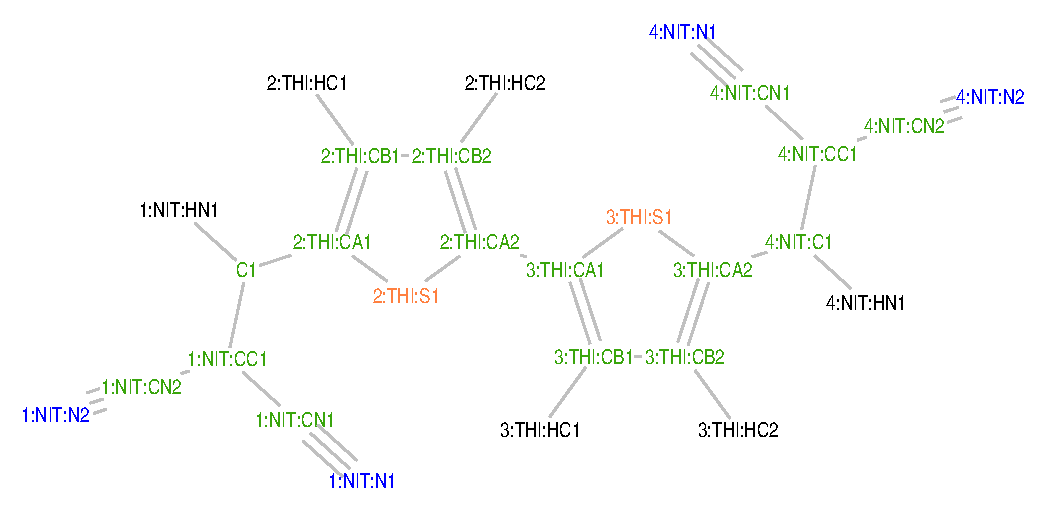
\includegraphics[width=0.8\textwidth]{./fig/chemical_structure/dcv2t_atom_types}
\caption{\small \dcvt with atoms labelled according to \texttt{residue\_number:residue\_name:atom\_name}. There are four residues and two residue types: thiophene (THI) and dicyanovinyl (NIT). The corresponding pdb file is shown in listing~\ref{list:pdb}.}
\label{fig:dcv2t_at}
\end{figure}

\lstinputlisting[
  language=XML,
  basicstyle=\ttfamily\small,
  stringstyle=\ttfamily\small,
  showstringspaces=false,
  frame=lines,
  label=list:pdb, 
  morekeywords={HETATM,THI,NIT},
  caption={\small pdb file of \dcvt.}]%
{./fig/chemical_structure/dcv2t.pdb}
\clearpage

\section{Mapping file}
\label{sec:xmlmap}
The mapping file (referred here as \xmlcsg) is used by the program \ctpmap to convert an atomistic trajectory to a trajectory with conjugated segments and rigid fragments. 
This trajectory is stored in a \slink{statefile}{state file} and contains positions, names, types of atoms belonging to rigid fragments. 
The description of the mapping options is given in table \ref{tab:map}. An example of \xmlcsg for a \dcvt molecule is shown in listing~\ref{list:map}. 
%
\begin{table}[h]
\label{tab:map}
\caption{Description of the \xml mapping file (\xmlcsg).}
\rowcolors{1}{invisiblegray}{white} {\footnotesize \input{reference/xml/map.xml}}
\end{table}
%
% Define new language for listings.
\lstdefinelanguage{MXML} {
   basicstyle=\ttfamily\scriptsize,
   sensitive=true,
   morecomment=[s][\color{gray}\rmfamily\itshape]{<!--}{-->}, 
   showstringspaces=false,
   numberstyle=\scriptsize,
   numberblanklines=true,
   showspaces=false,
   breaklines=true,
   showtabs=false,
   alsoletter={:},
   keywords = [1]
   { topology,molecules,molecule,name,mdname,segments,segment,fragments,fragment,mdatoms,qmatoms,localframe,weights},
   keywordstyle={[1]\color{blue}},
}

\lstinputlisting[
 language=MXML,
 label=list:map,
 caption={Examle of \xmlcsg for \dcvt. Each rigid fragment (coarse-grained bead) is defined by a list of atoms. Atom numbers, names, and residue names should correspond to those used in \gromacs topology (see the corresponing listing \ref{list:pdb} of the pdb file).}]%
{./input/dcv2t/map.xml}

\section{Conjugated segments}
\label{sec:xmlsegments}

The file describing hopping sites, or conjugated segments, is used by practically all programs and calculators. It links the coarse-grained trajectory (positions and orientations of rigid fragments) and quantum-mechanical descriptions of all conjugated segments. The description of this \xml file (\xmlsegments) is given in table \ref{tab:segments}. An example for \dcvt is shown in listing~\ref{list:segments}.

\begin{table}[h]
\caption{Description of conjugated segments (\xmlsegments).} 
\label{tab:segments}
\rowcolors{1}{invisiblegray}{white} {\small \input{reference/xml/segments.xml} }
\end{table}

\lstset{
  language=XML,
  frame=lines,
  basicstyle=\ttfamily\footnotesize,
  identifierstyle=\color{red},
  keywordstyle=\color{blue},
  showstringspaces=false,
  columns=fullflexible,
  commentstyle=\color{gray}\rmfamily\itshape,
  morekeywords={segments,segment,coordinates,orbitals,basisset,torbital,reorganization,qneutral,qcharged,energy,beadconj,molname,name,map,weights},
}

\lstinputlisting[
 label=list:segments, 
 caption={\small \xml file describing \slink{segments}{conjugated segments}. Note that the mapping and weights for each segment are separated by a colon. 
}]%
{./input/segments.xml}






\chapter{Manual pages}
%
% if you want to refer to any of the tags specified here use the following command
% \segmentopt{crgunit_type.ChargeUnitType.posname}
%
\section{Programs}
\label{ref:programs}
\input{reference/programs/all}

\section{Calculators}
\label{ref:calculators}
\label{sec:calculators}

Calculator is a piece of code which computes specific system properties, such as site energies, transfer integrals, etc. \ctprun is a wrapper program which executes all calculators. The generic syntax is 

  \ctprun \exe \texttt{"calc1, calc2, ..."} \opt \xmloptions
\vskip 0.2cm
%
File \xmloptions lists all options needed to run a specific calculator. The format of this file is explained in listing~\ref{list:calc}. A complete list of calculators is given in the \refcalc reference section.
%
\lstinputlisting[label=list:calc, 
 caption={\small A part of the \xmloptions file with options for the \texttt{calculator\_name\{1,2\}} \refcalc.
}]{./reference/calculators.xml}

\input{reference/calculators/all}
\vfill

\section{Options}
\label{ref:options}
%\setdefaultleftmargin{0.8em}{0.8em}{0.8em}{0.8em}{0.8em}{0.8em}

\subsection{Mapping file}
\rowcolors{1}{invisiblegray}{white}
{\small 
\input{reference/xml/map.xml}
}
\vfill

\subsection{Conjugated segments}
\rowcolors{1}{invisiblegray}{white}
{\small 
\input{reference/xml/segments.xml}
}
\vfill

\subsection{Calculator options}
\rowcolors{1}{invisiblegray}{white}
{\small 
\input{reference/xml/options.xml}
}
\vfill


\appendix
\newcommand{\indM}{l} 
\newcommand{\indN}{m}
\newcommand{\lb}[1]{\langle #1 |}
\newcommand{\rb}[1]{| #1 \rangle}
\newcommand{\rbt}[1]{ #1 \rangle}

%\appendixpage
%\addappheadtotoc
\chapter{Bimolecular electron transfer rate}

\begin{figure*}[ht]
%    \includegraphics[width=1.0\textwidth]{fig/jortner_rate/marcus_parabolas_new}
   \caption{
(a) Potential energy surfaces of the charge transfer complex in a dimer representation. ET is from molecule $i$ to molecule $j$. In the initial state, $\rb{I_{00}}$, both molecules are in their vibrational ground states. In the final state, $\rb{F_{l'm'}}$, the neutral molecule $i$ is in vibrational state $l'$, while the charged molecule $j$ is in vibrational state $m'$. Initial and final states are coupled to a classical harmonic outer-sphere normal mode with mass weighted average coordinate $q$ and reorganization energy $\lambda_{ij}^\text{out}$. For small couplings $V_{I_{00}F_{l'm'}}$ the ET reaction takes place on the diabatic states (solid curves). 
%
(b) PES of molecule $i$ as a function of the averaged normal mode $q_i$. $l$ and $l'$ enumerate vibrational modes of the initial charged and the final neutral states. (c) Same as (b) for initially neutral molecule $j$. 
%
$\Delta U_i$ ($\Delta U_j$) is the internal energy difference while $\lambda_i^{cn}$ ($\lambda_j^{nc}$) is the  intramolecular reorganization energy for discharging molecule $i$ (charging molecule $j$). }
   \label{fig:marcus_parabolas}
\end{figure*}

In the case of a bimolecular electron transfer (ET) reaction the electron moves between two independent molecules. Therefore, one needs separate sets of coordinates for the donor and acceptor. Strictly speaking, the classical Marcus rate assumes a common set of vibrational coordinates and, as such, can not be used for bimolecular ET. Yet if the independent vibrational modes are harmonic, are treated classically, and the charging and discharging reorganization energies of the molecule are identical, one still obtains the Marcus-type ET rate with the intramolecular reorganization energy which is the sum of the reorganization energies of the donor and the acceptor~\cite{may_charge_2003}. Similarly, the classical treatment of the outer-sphere mode, which is due to rearrangement of the surrounding, allows to add its reorganization energy  to the intramolecular one.

However, the main issue with the classical Marcus rate is that the high-frequency intramolecular vibrational modes are energetically comparable to the C-C bond stretching mode. At room temperature $\hbar \omega_\text{CC} \sim 0.2\, \unit{eV} \gg k_\text{B}T \sim 0.025\, \unit{eV}$  and therefore these modes should be treated quantum mechanically. In fact, for a common set of intramolecular high-frequency  (quantum-mechanical) and an outer sphere low-frequency (classical) vibrational coordinates, a mixed quantum-classical multi-channel generalization of the Marcus formula is readily available~\cite{may_charge_2003}. Such generalization,  to the best of our knowledge, has not been made for the bimolecular ET rate, which requires independent sets of coordinates for donor and acceptor. The purpose of this section is to derive a quantum-classical expression for the ET rate with two independent, high-frequency vibrational modes and a common low-frequency outer sphere mode. 

Following Ref.~\cite{bredas_charge-transfer_2004} we assume that all intramolecular modes of a donor $i$ can be averaged into a mode with mass weighted coordinate ${q_i}$ and energy $\hbar\omega^{n}_i$ ($\hbar\omega^{c}_i$) for the molecule in a neutral (charged) state. Similar assumptions are made for the acceptor $j$. In addition, we allow for an averaged classical outer-sphere mode with mass weighted coordinate ${q}$ and energy $\hbar\omega^\text{out}_{ij}\ll k_\text{B}T$. This mode is common to both molecules and plays the role of the ET reaction coordinate~\cite{note_outer}.

In amorphous organic semiconductors the electronic coupling is usually small compared to both the energy of the classical vibrational mode and intermolecular reorganization energies. In this case the initial, $ \rb{I_{\indM\indN}}$, and final, $\rb{F_{\indM'\indN'}}$, states of the ET reaction are diabatic (non-interacting) dimer states which depend on the vibrational states (with quantum numbers $\indM, \indN, \indM, '\indN'$) of both molecules. The potential energy surfaces (PES) corresponding to these states are shown in \fig{marcus_parabolas}a. The PES for intramolecular degrees of freedom for molecules $i$ and $j$ are shown in \fig{marcus_parabolas}b and c, respectively.

For the contributions of the outer-sphere mode to initial and final states we introduce Hamiltonian functions
\begin{equation}
 H_{I,F}(q)=\frac{1}{2}\left[ \omega^\text{out} \left( q-q_{I,F} \right) \right]^2 \, ,
\end{equation}
where the equilibrium position in the initial (final) state $q_I$ ($q_F$) corresponds to the arrangement of all nuclear coordinates of molecules surrounding the ET complex when molecule $i$ ($j$) is charged.  The outer sphere reorganization energy, defined as $\lambda^\text{out}_{ij}=\frac{1}{2}\left[ \omega^\text{out}|q_I-q_F| \right]^2$,  is shown in~\fig{marcus_parabolas}a. It can be computed from the initial and final electric displacement fields of the charge-transfer complex. 

The complete Hamiltonian of the ET complex can now be written as
\begin{equation}
\begin{split}
 H_{ij}=&\hphantom{+}\sum_{\indM,\indN=0}^\infty \left( H_I(q) + E^{ij}_{\indM\indN} \right) \rb{I_{\indM\indN}} \lb{I_{\indM\indN}} %\\
        +\sum_{\indM',\indN'=0}^\infty \left( H_F(q) + E^{ji}_{\indN'\indM'} \right) \rb{F_{\indM'\indN'}} \lb{F_{\indM'\indN'}} %\\
        +\sum_{\indM,\indN,\indM',\indN'}V_{I_{\indM\indN}F_{\indM'\indN'}} \rb{I_{\indM\indN}} \lb{F_{\indM'\indN'}} +\text{h.c} \,, \\
 E^{ij}_{\indM\indN}=& \hphantom{+} U_i^{cC} + U_j^{nN} + E_i^\text{el} + E_i^\text{ext}
+ \hbar\left[\omega_i^c\left(\indM+\frac{1}{2}\right) + \omega_j^n\left(\indN+\frac{1}{2}\right) \right] \, , 
       \\
 E^{ji}_{\indN'\indM'}=&\hphantom{+} U_j^{cC} + U_i^{nN} + E_j^\text{el} + E_j^\text{ext} 
+ \hbar\left[\omega_j^c\left(\indN'+\frac{1}{2}\right) +\omega_i^n\left(\indM'+\frac{1}{2}\right)\right] \, .
\end{split}
\label{equ:hami}
\end{equation}
Here, a manifold of initial states, $\rb{I_{\indM \indN}} $, with quantum numbers $\indM$ ($\indN$) for intramolecular vibrations in molecule $i$ ($j$) and energy $E^{ij}_{\indM \indN}$, is coupled to a classical phonon bath $H_I(q)$. Transitions to the manifold of final states  $\rb{F_{\indM' \indN'}} $ where the charge has hopped from $i$ to $j$ are possible due to a coupling $V_{I_{\indM\indN}F_{\indM'\indN'}} $.
The initial, $E^{ij}_{\indM\indN}$,  and final, $E^{ji}_{\indN'\indM'}$, energies contain internal energies $U_i^{nN}$ and $U_i^{cC}$ ($U_j^{nN}$ and $U_j^{cC}$) of molecule $i$ (molecule $j$) in the neutral and charged ground states, the contributions of the external electric field, $E_i^\text{ext}$ and $E_j^\text{ext}$, and electrostatic interactions, $E_i^\text{el}$ and $E_j^\text{el}$, and respective oscillator energies.  

Within the Born-Oppenheimer approximation, a separation in terms of electronic and nuclear degrees of freedom gives
\begin{equation}
\begin{split}
 \rb{I_{\indM\indN}}&=\rb{\phi_i^c}\rb{\chi_{i\indM}^c}\rb{\phi_j^n}\rb{\chi^n_{j\indN}}\, ,\\
 \rb{F_{\indM'\indN'}}&=\rb{\phi^n_i}\rb{\chi^n_{i\indM'}}\rb{\phi_j^c}\rb{\chi_{j\indN'}^c}\, ,
\end{split}
\end{equation}
where $\phi_i^n$ ($\phi_i^c$) corresponds to the electronic part of the wave function, while $\chi_{i\indM}^n$  ($\chi_{i\indM}^c$) represents an $\indM$-th phonon mode of the neutral (charged) molecule $i$.

The coupling element $V_{I_{\indM\indN}F_{\indM'\indN'}}$ in~\equ{hami} can then be factorized in an electronic and nuclear parts 
\begin{equation}
V_{I_{\indM\indN}F_{\indM'\indN'}}=J_{ij} \lb{\chi_{i\indM}^c}\rbt{\chi_{i\indM'}^n} \lb{\chi_{j\indN}^n}\rbt{\chi_{j\indN'}^c}\,.
\end{equation}
Franck-Condon overlap integrals $\lb{\chi_{i\indM}^c}\rbt{\chi_{i\indM'}^n}$ ($\lb{\chi_{j\indN}^n}\rbt{\chi_{j\indN'}^c} $) describe couplings of vibrational modes $\indM,\indM'$ ($\indN,\indN'$) of the charged and neutral configurations of molecule $i$  ($j$). Exemplary modes are shown in~\fig{marcus_parabolas}b,c.

Since $k_\text{B}T\ll \hbar\omega_i^{c},\hbar\omega_j^{n}$ one can restrict the initial state to the vibrational ground-states $\indM=\indN=0$ while allowing tunneling to all vibrationally excited states $\indM'$ for molecule $i$ and $\indN'$ for molecule $j$. In other words, a single initial state $\rb{I_{00}}$ couples to a manifold of final states $\rb{F_{\indM',\indN'}}$. 
%
This assumes that ET is sufficiently slow compared to the relaxation of the intramolecular degrees of freedom, so that there is enough time for a complex to relax to its vibrational ground state between two consecutive ETs. 

The energy difference driving the reaction to channel ${\indM'\indN'}$  therefore is
\begin{equation*}
 \Delta E^{ij}_{\indM'\indN'}= E^{ij}_{00}-E^{ji}_{\indN'\indM'}=\Delta E_{ij} - \hbar (\omega_i^n\indM'+\omega_j^c\indN')\,,
\end{equation*}
where $\Delta E_{ij}=\Delta E_{ij}^\text{ext}+\Delta E_{ij}^\text{el}+\Delta E^\text{int}_{ij}$.

Assuming that $|V_{I_{00}F_{\indM'\indN'}}|\ll\lambda_{ij}^\text{out},\hbar\omega^\text{out}$ and using Fermi's golden rule with $V_{I_{00}F_{\indM'\indN'}}$ as a perturbation to the initial diabatic state, we obtain a multi-channel rate equation
\begin{equation}
%\begin{split}
\omega_{ij}=\sum_{\indM',\indN'=0}^\infty \frac{2\pi}{\hbar}|V_{I_{00}F_{\indM'\indN'}}|^2 
% \times  
\int dq f_I(q) \delta(\Delta E^{ij}_{\indM'\indN'} + H_I(q) -H_F(q))\, .
%\end{split}
\end{equation}
where the thermal averaging over the classical outer-sphere mode is performed by introducing a  canonical distribution function  $f_I(q)=Z^{-1}\exp(-H_I(q)/k_\text{B}T)$, with $Z=\int{dq \exp(-H_I(q)/k_\text{B}T)}$.

Energy conservation pins the transition to the crossing point of the diabatic PES (see~\fig{marcus_parabolas}a) resulting in 
\begin{eqnarray}
 \omega_{ij}= \frac{2\pi}{\hbar}  \frac{|J_{ij}|^2}{\sqrt{4\pi \lambda_{ij}^\text{out} k_\text{B}T}} 
 \sum_{\indM',\indN'=0}^\infty
 |\lb{\chi_{i0}^c}\rbt{\chi_{i\indM'}^n}|^2 |\lb{\chi_{j0}^n}\rbt{\chi_{j\indN'}^c}|^2 
%\nonumber \\&& 
\exp
\left\{ -\frac{ \left[ \Delta E_{ij}-\hbar(\indM'\omega_i^n+\indN'\omega_j^c) -\lambda_{ij}^\text{out} \right]^2}{4\lambda_{ij}^\text{out} k_\text{B}T}
\right\} .
\label{equ:jjortner}
\end{eqnarray}
\Equ{jjortner} is the quantum-classical expression for the bimolecular ET rate with two independent, high-frequency vibrational modes and one classical common outer-sphere mode. It is the main result of this section. 

If the curvatures of intramolecular PES of charged and neutral states of a molecule are different, that is $\omega_i^c\neq\omega_i^n$, the corresponding reorganization energies, $\lambda_i^{cn}=\frac{1}{2}[\omega_i^n(q_i^n-q_i^c)]^2$ and $\lambda_i^{nc}=\frac{1}{2}[\omega_i^c(q_i^n-q_i^c)]^2$, will also differ. In this case the Franck-Condon (FC) factors for discharging of molecule $i$ read \cite{chang_new_2005}
\begin{equation}
%\begin{split}
%&
|\lb{\chi_{i0}^c}\rbt{\chi_{i\indM'}^n}|^2 = 
\frac{2}{2^{l'}l'!} \frac{\sqrt{\omega_i^c\omega_i^n}}{(\omega_i^c+\omega_i^n)} \exp\left( -|s_i| \right)
%\nonumber \\
%& \times
 \left[ \sum_{\substack{k=0\\k\,\text{even}}}^{\indM'} {\indM' \choose k} 
\left( \frac{2 \omega_i^c }{\omega_i^c+\omega_i^n}\right)^{k/2} \frac{k!}{(k/2)!}
H_{\indM'-k} \left( \frac{s_{i}}{\sqrt{2S^{cn}_i}}\right) 
\right]^2
\, ,
%\end{split}
\end{equation}
where $H_n(x)$ is a Hermite polynomial, $s_i=\frac{2\sqrt{\lambda_i^{nc}\lambda_i^{cn}}}{\hbar(\omega_i^c+\omega_i^n)}$, and $S^{cn}_i=\lambda_i^{cn}/\hbar\omega_i^c$. The FC factors for charging of molecule $j$ can be obtained by substituting $(s_i,S^{cn}_i,\omega_i^c)$ with $(-s_j,S^{nc}_j, \omega_j^n)$. In order to evaluate the FC factors, the internal reorganization energy $\lambda_i^{cn}$ can be computed from the intramolecular PES, as shown in~\fig{marcus_parabolas}b,c. 

To conclude the section, we compare the bimolecular quantum-classical rate, \equ{jjortner}, the classical bimolecular Marcus rate, eq.~(1) of the main text, and the quantum-classical Jortner rate with a common set of vibrational coordinates~\cite{may_charge_2003}
\begin{eqnarray}
 \omega_{ij} = \frac{2\pi}{\hbar}  \frac{|J_{ij}|^2}{\sqrt{4\pi \lambda_{ij}^\text{out} k_\text{B}T}} 
 \sum_{N=0}^\infty \frac{1}{N!} \left( \frac{\lambda_{ij}^\text{int}}{\hbar\omega^\text{int}} \right)^{N} 
  \exp \left( - \frac{\lambda_{ij}^\text{int}}{\hbar\omega^\text{int}}\right) 
%\nonumber\\&& 
\exp
\left\{ -\frac{ \left[ \Delta E_{ij}-\hbar N\omega^\text{int} -\lambda_{ij}^\text{out} \right]^2}{4\lambda_{ij}^\text{out} k_\text{B}T}
\right\} .
\label{equ:jortner}
\end{eqnarray}

If $\omega_i^c=\omega_i^n=\omega_i$ ($\lambda_i^{nc}=\lambda_i^{cn}=\lambda_i$), the Franck-Condon factor simplifies to
\begin{equation}
|\lb{\chi_{i0}}\rbt{\chi_{i\indM'}}|^2 = \frac{1}{\indM'!} \left( \frac{\lambda_i}{\hbar\omega_i} \right)^{\indM'} \exp \left( - \frac{\lambda_i}{\hbar\omega_i}\right)\,.
\end{equation}
If this simplification is applicable for both donor and acceptor molecules,  \equ{jjortner} becomes identical to the quantum-classical rate~\equ{jortner} with $\lambda_{ij}^\text{int}=\lambda_i+\lambda_j$.

\begin{figure*}[ht]
%   \includegraphics[width=\linewidth]{fig/jortner_rate/compare_rates}
   \caption{ (a) Scaled hopping rates, $\bar{\omega}_{ij} = \omega_{ij}  J_{ij}^{-2} (2\pi)^{-1} \hbar\sqrt{4\pi k_\text{B}T}$, calculated using the classical Marcus, Jortner quantum mechanical~\equ{jortner} and bimolecular multichannel~\equ{jjortner} rate expressions. 
%
Outer sphere reorganization energy $\lambda_{ij}^\text{out}=0.05\, \unit{eV}$,  $\lambda^{cn}_i=\lambda_j^{cn}=0.14\, \unit{eV}$, and $\lambda^{nc}_i=\lambda^{nc}_j=0.09\, \unit{eV}$ (all added in the classical Marcus rate while the latter two are added for the Jortner rate). 
%
Intramolecular vibrations have averaged frequency $\hbar\omega_i^\text{int}=\hbar\omega_j^\text{int}=0.2\, \unit{eV}$ for the Jortner rate while $\hbar\omega_i^n=0.2\, \unit{eV}$ and $\hbar\omega_j^c=\hbar\omega_i^n \sqrt{\lambda_j^{nc}}/\sqrt{\lambda_j^{cn}}$ for the bimolecular rate. 
%
(b) The same but for $\lambda_{ij}^\text{out}=0.1\, \unit{eV}$. 
%
(c) Histogram of rates at a field of $10^8\, \unit{Vm^{-1}}$ for the Marcus and Jortner rates with distance dependent $\lambda_{ij}^\text{out}<0.08\, \unit{eV}$ for the neighborlist pairs and constant $\lambda^\text{int}=0.23\, \unit{eV}$. A small difference can be seen in the tail of small rates.}
   \label{fig:mj_comparison}
\end{figure*}

% discussion of the equation
To compare the quantum-mechanical and classical rates, intramolecular hole reorganization energies of \Alq, $\lambda^{cn}_i=0.14\,\unit{eV}$ and $\lambda^{nc}_i=0.09\,\unit{eV}$ were used. We also assumed that $\omega_i^n=0.2\,\unit{eV}$ and $\omega_i^c=\omega_i^n\sqrt{\lambda^{nc}_i / \lambda^{cn}_i}$. Due to the uncertainty in determining $\lambda_{ij}^\text{out}$, two cases are considered, $\lambda_{ij}^\text{out}=0.05\,\unit{eV}$ (\fig{mj_comparison}a) and $\lambda_{ij}^\text{out}=0.10\,\unit{eV}$ (\fig{mj_comparison}b). Note that the estimate made in the main text predicts $\lambda_{ij}^\text{out} < 0.08\,\text{eV}$. In both cases we used fixed, molecular-separation independent, $\lambda_{ij}^\text{out}$. 

\Fig{mj_comparison} shows that the main difference between the quantum-classical and classical rates is the tail of smaller rates for large negative $\Delta E$ (endothermal hopping) and higher rates for large positive $\Delta E$ (exothermal hopping).  \Fig{mj_comparison}c also shows the corresponding distributions of rates for all pairs from the neighbor list for 512 molecules of  amorphous \Alq. Here we used the distance-dependent $\lambda_{ij}^\text{out}$ from the neighbor list as computed from dielectric displacement fields with the Pekar factor of $c_p=0.01$. One can see that the distributions are practically on top of each other (except for very small rates) and hence will lead to similar charge dynamics. 

In general, our observation is that for a situation with (i) intramolecular reorganization energy similar to the outer sphere one ($\lambda_{ij}^\text{int} \sim \lambda_{ij}^\text{out}$), (ii) driving force $\Delta E_{ij}$ small compared to the intramolecular reorganization energy, and (iii) $\lambda \sim \hbar \omega$, the classical (eq.~(1) of the main text) and semi-classical  (\equ{jortner} and \equ{jjortner}) expressions lead to quantitatively similar rates.
However, for systems with large $\Delta E_{ij}$, such as donor-acceptor mixtures, \equ{jjortner} or \equ{jortner} should be used. In this case a rather accurate estimate of the outer sphere reorganization energy is required~\cite{mcmahon_evaluation_2010}.


\subsection{Calculators}
\label{sec:calculators}

\ctprun is a wrapper program which is used to run all calculators. The generic syntax is 
\begin{verbatim}
  ctp_run --exec "calc1, calc2, ..." --opt options.xml
\end{verbatim}
%
File \texttt{options.xml} lists all options needed to run a specific calculator. The format of this file is explained in listing~\ref{list:calc}. A complete list of calculators is given in the \refcalc reference section.
%
\lstinputlisting[label=list:calc, 
 caption={\small Part of the \texttt{options.xml} file with options for the \texttt{calculator\_name} \refcalc.
}]{./programs/calculators.xml}


\bibliographystyle{achemso}
\bibliography{literature_short}

\end{document} 
